\documentclass[a4paper, twoside, table, justified,
               nofonts, nobib, nohyper, 10pt, french]{tufte-book}

%!TEX root = ../main.tex

%% ==============================================================
%% Encoding

\usepackage[french]{babel}
\usepackage[utf8]{inputenc}
\usepackage[T1]{fontenc}

%% ==============================================================
%% Title page style

%% INPT / Toulouse University title page
\usepackage[ED=MITT-SIAO, Ets=INP]{tlsflyleaf}

% \usepackage{lmodern}\normalfont
% \DeclareFontShape{T1}{lmr}{bx}{sc}{ <-> ssub * cmr/bx/sc }{}
% \DeclareOldFontCommand{\bf}{\normalfont\bfseries}{\mathbf}
% \usepackage[osf,sc]{mathpazo}

%% Setup basic string
\title{Acquisition rapide et reconstruction en imagerie EELS.}
%
\author{Etienne Monier}
%
\defencedate{??/??/????}
%
\lab{Institut de Recherche en Informatique de Toulouse (UMR 5505)}

%% Boss
\nboss{2}
%
\makesomeone{boss}{1}{Nicolas \textsc{Dobigeon}}{Professeur à l'INP-ENSEEIHT}{Directeur de thèse}
\makesomeone{boss}{2}{Thomas \textsc{Oberlin}}{Maître de conférence à l'INP-ENSEEIHT}{Co-directeur de thèse}

%% Referee
\nreferee{2}
\makesomeone{referee}{1}{? \textsc{?}}{?}{Rapporteur}
\makesomeone{referee}{2}{? \textsc{?}}{?}{Rapporteur}

%% Judges
\njudge{7}
\makesomeone{judge}{1}{? \textsc{?}}{?}{Rapporteur}
\makesomeone{judge}{2}{? \textsc{?}}{?}{Rapporteur}
\makesomeone{judge}{3}{? \textsc{?}}{?}{Examinateur}
\makesomeone{judge}{4}{? \textsc{?}}{?}{Examinateur}
\makesomeone{judge}{5}{? \textsc{?}}{?}{Examinateur}
\makesomeone{judge}{6}{Nicolas \textsc{Dobigeon}}{Professeur à l'INP-ENSEEIHT}{Directeur de thèse}
\makesomeone{judge}{7}{Thomas \textsc{Oberlin}}{Maître de conférence à l'ISAE-SUPAERO}{Co-directeur de thèse}


%% ==============================================================
%% Warning filtering

\usepackage{silence}
%\WarningFilter{biblatex}{Patching footnotes failed}
%\WarningFilter{biblatex}{Attempt to redefine deprecated}
\WarningFilter{latex}{Marginpar on page}
\WarningFilter{latexfont}{Font shape}
\WarningFilter{latexfont}{Some font}
\WarningFilter{latexfont}{Size substitutions}

%% ==============================================================
%% Index

% Generates the index https://en.wikibooks.org/wiki/LaTeX/Indexing
% https://www.overleaf.com/learn/latex/Indices
% To make clickable links with hyperref
% pass nohyper option to tufte documentclass
% and load hyperref after imakeidx
\usepackage{imakeidx}
\indexsetup{level=\chapter*, toclevel=chapter}
\makeindex[title=Index, columns=1, intoc]

%% ==============================================================
%% Hyperef links

\usepackage[svgnames]{xcolor}
\definecolor{mydarkblue}{rgb}{0,0.08,0.45}
\definecolor{myblue}{RGB}{18,75,126}
\definecolor{burgundy}{RGB}{128,0,32}

\usepackage{hyperref}
\hypersetup{
    linktoc=all,
    breaklinks=true,
    colorlinks=true,
    linkcolor=mydarkblue,
    citecolor=mydarkblue,
    filecolor=mydarkblue,
    urlcolor=mydarkblue
}


%% ==============================================================
%% Glossary

% https://www.overleaf.com/learn/latex/Glossaries
% Terminal: makeglossaries main
% rebuild main.tex
% To make clickable links with hyperref
% load hyperref before glossaries

% Some lengths
\TufteRecalculate
\newlength\fullwidthwidth
\makeatletter\setlength\fullwidthwidth{\@tufte@fullwidth}\makeatother

\newlength\centralcol
\setlength\centralcol{\fullwidthwidth}
\addtolength{\centralcol}{-5cm}

% Glossaries input.
\usepackage[%
    % nopostdot,  % If no final point is desired for description.
    nonumberlist,  % The location should not be displayed.
    acronym,
    toc,
    section=subsection,  % Sets the printglossaries be a section.
    numberedsection=false,  % To have section* instead of section.
    nogroupskip=true,
    xindy,
    ucmark,
    shortcuts]{glossaries}

%
% New gloassaries
%

% Adds a key to glossaries entries
\glsaddstoragekey{shape}{}{\glsshape}

% Add all entries into list


% Glossaries sections
\newglossary[nglg]{notgen}{nge}{ngtn}{Notations générales}
\newglossary[nlg]{notation}{not}{ntn}{Notations}

%
% Format
%

% Defines the accronym display style. Long desc. first, then short one.
\setacronymstyle{long-short}

% Removes space after section name
\renewcommand{\glossarypreamble}{\vspace*{-\baselineskip}}

% This command disables hyperlinks from text to glossary list.
\glsdisablehyper

% https://tex.stackexchange.com/questions/269565/glossaries-how-to-customize-list-of-symbols-with-additional-column-for-units

%\setlength\centralcol{10cm minus 1.5cm minus 1.5cm}
\newglossarystyle{symbunitlong}{%
    \setglossarystyle{long3col}% base this style on the list style
    \renewenvironment{theglossary}{% Change the table type --> 3 columns
        \begin{longtable}{p{1.5cm}p{\centralcol}>{\hfill}p{1.5cm}}}%
        {\end{longtable}}%
    %
%    \renewcommand*{\glossaryheader}{%  Change the table header
%        \bfseries Sign & \bfseries Description & \bfseries Unit \\
%        \hline
%        \endhead}
    \renewcommand*{\glossentry}[2]{%  Change the displayed items
        \glstarget{##1}{\glossentryname{##1}} %
        & \glossentrydesc{##1}% Description
        & \glsshape{##1}  \tabularnewline
    }
}

\newglossarystyle{acrolong}{%
    \setglossarystyle{long3col}% base this style on the list style
    \renewenvironment{theglossary}{% Change the table type --> 3 columns
        \begin{longtable}{p{1.5cm}p{\textwidth-1.5cm}}}%
        {\end{longtable}}%
    %
    %    \renewcommand*{\glossaryheader}{%  Change the table header
    %        \bfseries Sign & \bfseries Description & \bfseries Unit \\
    %        \hline
    %        \endhead}
    \renewcommand*{\glossentry}[2]{%  Change the displayed items
        \glstarget{##1}{\glossentryname{##1}} %
        & \glossentrydesc{##1}% Description
        \tabularnewline
    }
}


%
% Starts glossaries and input entries
%

\makeglossaries

%!TEX root = ../main.tex
% To build the glossary: makeglossaries main

%%%%% Acronyms
% \newacronym[plural={<plural acronym>},
%             first={<text displayed at first occurrence>},
%             firstplural={<idem, with plural>}]
%             {<label>}
%             {<acronym>}
%             {<full name to display in acronym section>}

% Laboratoires
\newacronym{irit}
           {IRIT}
           {Institut de Recherche en Informatique de Toulouse}

\newacronym{lps}
           {LPS}
           {Laboratoire de Physique des Solides}

% Microscopes
\newacronym{stem}
           {STEM}
           {Scanning Transmission Electron Microscope}

\newacronym{tem}
           {TEM}
           {Transmission Electron Microscope}

\newacronym{sem}
           {SEM}
           {Scanning Electron Microscope}

\newacronym{mfa}
           {MFA}
           {microscopie à force atomique}

% Modalités
\newacronym{haadf}
           {HAADF}
           {High-Angle Annular Dark-Field}

\newacronym{eels}
           {EELS}
           {Electron Energy Loss Spectroscopy}

\newacronym{edx}
           {EDX}
           {analyse dispersive en énergie}


% Techniques
\newacronym{pca}
           {ACP}
           {Analyse par Composantes Principales}

\newacronym{cs}
           {CS}
           {Compressed Sensing}

\newacronym{ppv}
           {PPV}
           {Plus Proches Voisins}

\newacronym{ad}
           {AD}
           {Apprentissage de Dictionnaire}

\newacronym{ebi}
           {EBI}
           {Exemplar-Based Inpainting}

\newacronym{mc}
           {MC}
           {moindre carré}
        
\newacronym{dct}
           {DCT}
           {transformée en cosinus discrète}

\newacronym{tv}
           {TV}
           {variation totale}

%%%% Glossary entries


%% Notations génériques

\newglossaryentry{g-a}{type=notgen, name={\ensuremath{a}}, description={Scalaire}, sort={01}}

\newglossaryentry{g-av}{type=notgen,
	name={\ensuremath{\mathbf{a}}},
	description={Vecteur colonne}, 
	sort={02}}

\newglossaryentry{gavi}{type=notgen, 
	name={\ensuremath{\mathbf{a}_i}}, 
	description={$i^\text{ème}$ composante du vecteur \gls{g-av}}, 
	sort={03}}

\newglossaryentry{g-A}{type=notgen, 
	name={\ensuremath{\mathbf{A}}},
	description={Matrice},
	sort={04}}

\newglossaryentry{g-Aij}{type=notgen,
	name={\ensuremath{\mathbf{A}_{ij}}},
	description={Coefficient $(i, j)$ de la matrice \gls{g-A}},
	sort={05}}

\newglossaryentry{g-Aj}{type=notgen, 
	name={\ensuremath{\mathbf{A}_j}},
	description={$j^\text{ème}$ colonne de la matrice \gls{g-A}},
	sort={06}}

\newglossaryentry{g-Ai}{type=notgen, 
	name={\ensuremath{\mathbf{A}_{i, :}}},
	description={$i^\text{ème}$ ligne de la matrice \gls{g-A}},
	sort={07}}

\newglossaryentry{g-T}{type=notgen, 
	name={\ensuremath{(\cdot)^{T}}},
	description={Transposée},
	sort={08}}

\newglossaryentry{g-pm}{type=notgen, 
	name={\ensuremath{\mathbf{AB}}},
	description={Produit matriciel},
	sort={09}}

\newglossaryentry{g-nf}{type=notgen, 
	name={\ensuremath{||\mathbf{A}||_F}},
	description={Norme de Frobenius de \gls{g-A}},
	sort={10}}



%% Dimensions
\newglossaryentry{P}{
	type=notation,
	name={\ensuremath{P}},
	description={Le nombre de pixels},
	sort={01}
}

\newglossaryentry{M}{
	type=notation,
	name={\ensuremath{M}},
	description={Le nombre de cannaux},
	sort={02}
}

\newglossaryentry{N}{
	type=notation,
	name={\ensuremath{N}},
	description={Le nombre de pixels acquis},
	sort={03}
}

\newglossaryentry{r}{
	type=notation,
	name={\ensuremath{r}},
	description={Le rapport d'acquisition $\gls{N}/\gls{P}$},
	sort={04}
}

%% Variance
\newglossaryentry{sig}{
	type=notation,
	name={\ensuremath{\sigma}},
	description={La variance du bruit blanc additif gaussien},
	sort={05}
}

%% Sets
\newglossaryentry{I}{
	type=notation,
	name={\ensuremath{\mathcal{I}}},
	description={L'ensemble des index des positions spatiales acquises},
	shape={(\gls{N}, )},
	sort={06}
}

%% Matrices
\newglossaryentry{X}{
	type=notation,
	name={\ensuremath{\mathbf{X}}},
	description={Les données inconnues à restituer},
	shape={(\gls{M}, \gls{P})},
	sort={07}
}

\newglossaryentry{Y}{
	type=notation,
	name={\ensuremath{\mathbf{Y}}},
	description={La matrice d'observation},
	shape={(\gls{M}, \gls{N})},
	sort={08}
}

\newglossaryentry{B}{
	type=notation,
	name={\ensuremath{\mathbf{B}}},
	description={La matrice de bruit gaussien},
	shape={(\gls{M}, \gls{N})},
	sort={09}
}

\newglossaryentry{Xh}{
    type=notation,
    name={\ensuremath{\hat{\mathbf{X}}}},
    description={Les données reconstruites},
    shape={(\gls{M}, \gls{P})},
    sort={10}
}





%% ==============================================================
%% Nomenclature

% to build nomenclature
% makeindex main.nlo -s nomencl.ist -o main.nls
% rebuild main.tex
\usepackage[intoc]{nomencl}
\makenomenclature
% \nomlabelwidth=30mm
\setlength{\nomitemsep}{.5\parsep}
\renewcommand{\nomname}{Notations}
%\newcommand{\nomunit}[1]{%
%\renewcommand{\nomentryend}{\hspace*{\fill}#1}}

\usepackage{etoolbox}  % required in nomenclature.tex

%% ==============================================================
%% Subappendix

% Add appendix to each chapter
\usepackage[toc,page]{appendix}
\usepackage{chngcntr}

\AtBeginEnvironment{subappendices}{%
    \newpage
    \section*{Appendices}
    \phantomsection
    \addtocontents{toc}{\vspace{1ex}} % small vertical space
    \addtocontents{toc}{\protect\contentsline{section}{\protect\textsc{Appendices}}{}{}}
    \counterwithin{equation}{section}
    \counterwithin{figure}{section}
    \counterwithin{table}{section}
}
\AtEndEnvironment{subappendices}{%
    \counterwithin{equation}{section}
    \counterwithout{figure}{section}
    \counterwithout{table}{section}
}

%% ==============================================================
%% Style de page

\renewcommand\chaptermark[1]{\markboth{\chaptername\thechapter. #1}{}}
\renewcommand\sectionmark[1]{\markright{\thesection. #1}}

\usepackage[fit]{truncate}
\newcommand{\markformat}[1]{\truncate{0.95\textwidth}{\footnotesize\scshape\nouppercase{#1}}}

\renewcommand\frontmatter{%
    \cleardoublepage%
    \pagenumbering{roman}%
    %\pagestyle{plain}%
    \fancyhf{}%
    \ifthenelse{\boolean{@tufte@twoside}}%
    {\fancyhead[LE,RO]{\thepage}}%
    {\fancyhead[RE,RO]{\thepage}}%
}

\renewcommand\mainmatter{%
    \cleardoublepage%
    \pagenumbering{arabic}%
    \fancyhf{}%
%    \renewcommand{\chaptermark}[1]{\markboth{##1}{}}%
%    \fancyhead[LE]{\thepage\quad\smallcaps{\newlinetospace{\plaintitle}}}% book title
%    \fancyhead[RO]{\smallcaps{\newlinetospace{\leftmark}}\quad\thepage}% chapter title
\fancyhead[LO]{\markformat{\rightmark}}
\fancyhead[RE]{\markformat{\leftmark}}
\fancyhead[LE, RO]{\footnotesize\thepage}
}

\usepackage{fancyhdr}
% \pagestyle{fancy}

\RequirePackage{etoolbox}                                                   
\appto\frontmatter{\pagestyle{fancy}}                                       
\appto\mainmatter{\pagestyle{fancy}}                                        
\appto\backmatter{\pagestyle{empty}} 

% \fancyhf{}



%% ==============================================================
%% Text packages

\usepackage{xcolor}  % Colors
\usepackage{enumerate}
\usepackage[shortlabels]{enumitem}       % personnalisation des enumerate
\setlist[itemize]{label=$\square$}  % black

%% ==============================================================
%% Graphics packages

% Figure / Float
% \usepackage{float}      % Ability to define new figure style, proposes H as a position.
% \usepackage[caption=false]{subfig}     % Create subfloats with \subfloat[caption]{figure}
% or \subtable[caption]{figure}
% \usepackage{subfloat}
% \usepackage[export]{adjustbox}  % To use \vphantom for vertical alignment of subfloat.


% Include graphic
\usepackage{graphicx}
\DeclareGraphicsExtensions{.pdf,.jpg,.png}
\graphicspath{{img/}}

\usepackage[center]{subfigure}

% Tikz config
\usepackage{style/tikzstyle}

%% ==============================================================
%% Math packages

%% Math symbols and font
\usepackage{amsmath}    % Main commands.
\usepackage{amssymb}    % Main symbols
\usepackage{dsfont}     % \mathds{1} pour indicatrice
\usepackage{amsfonts}
\usepackage{amsthm}
\usepackage{mathrsfs}   % Ralph Smith’s Formal Script Font : mathscr{A}
\usepackage{mathtools}  % \DeclarePairedDelimiter{\ceil}{\lceil}{\rceil}
\usepackage{stmaryrd}   % \llbracket et \rrbracket %sinon : $[\![$ et $]\!]$

%% Algorithms
\usepackage[ruled,vlined]{algorithm2e} % package environnement algorithme

%% Theorems and definitions
\newtheorem{mydef}{Définition}

%\usepackage{tcolorbox}
%\tcbuselibrary{skins}
%\tcbuselibrary{theorems}
%
%\newtcbtheorem[number within=chapter]{definition}{Définition}{%
%colbacktitle=gray!40, colback=gray!20, boxrule=0pt, fonttitle=\bfseries,%
%arc=0pt,outer arc=0pt%
%}{definitionlabel}


%% ==============================================================
%% Tabular packages

\usepackage{tabularx}
\usepackage{multirow}
\usepackage{booktabs}     % For serious tables (\toprule, \midrule, \bottomrule).


%% ==============================================================
%% FontAwesome

\usepackage{pgffor}
\usepackage{fontawesome}

\newcommand{\minusfa}[1][1]{%
    \foreach \n in {1,...,#1}{\color{red}\faicon{minus-square}}%
}
\newcommand{\plusfa}[1][1]{%
    \foreach \n in {1,...,#1}{\color{green}\faicon{plus-square}}%  plus plus-square plus-circle
}
\newcommand{\checkfa}{{\color{black}\faicon{check-square}}}  % check check-square check-circle

%% ==============================================================
%% Pretty refs

\usepackage[noabbrev]{cleveref}


\usepackage[]{todo}
\renewcommand\todoformat{\bfseries\small\color{red}}

\newcommand{\mref}{{\bfseries\color{red}[REF]}}
% \usepackage{showframe}


%% ==============================================================
%% Correct label

%\let\oldlabel\label
%\renewcommand{\label}[1]{\protect\oldlabel{#1}}
%
%% margincaption, leftbody, ragged, wide
%\usepackage[rightcaption, ragged, margincaption]{sidecap}
%\sidecaptionvpos{figure}{t} 
%\sidecaptionvpos{table}{t}
%
%\usepackage{floatrow}
%\DeclareFloatSeparators{mcapwidth}{\begingroup\hspace{\marginparsep}\endgroup}
%\floatsetup[widefigure]{margins=hangright,capposition=beside,
%    capbesideposition={top,right},floatwidth=\textwidth, capbesidewidth=\marginparwidth}, capbesidesep=mcapwidth}
%


\usepackage{lipsum}
\usepackage{comment}

\usepackage{showframe}


\begin{document}

%%%%%%%%%%%%%%%%%%%%%%%%%%%%%%%%%%%%%%%%%%%%%%%%%%%%%%%%%%%%%%%%%%%%%%%%%%%%
% The front matter contains title page, acknowledgements, toc, nomenclature and dedication
%%%%%%%%%%%%%%%%%%%%%%%%%%%%%%%%%%%%%%%%%%%%%%%%%%%%%%%%%%%%%%%%%%%%%%%%%%%%

\makeflyleaf
\frontmatter

\setcounter{chapter}{-1}
\setcounter{secnumdepth}{3}
\setcounter{tocdepth}{1}


%
% Remerciements
%

%!TEX root = ../main.tex

\chapter*{Remerciements} % (fold)
\label{ch:remerciements}

    Je remercie chalereusement \dots
    
    \lipsum[1-3]

% chapter remerciements (end)


%
% Dédicace
%

%!TEX root = ../main.tex

\clearpage
~\vfill
\thispagestyle{plain}
\begin{doublespace}
    \noindent\fontsize{18}{22}\selectfont\itshape
    \nohyphenation
    To ...
\end{doublespace}
\vfill
\vfill


%
% Table des matières
%

\begin{fullwidth}
    \tableofcontents
\end{fullwidth}


%
% Notations
%

%!TEX root = ../main.tex
% to build nomenclature
% makeindex main.nlo -s nomencl.ist -o main.nls
% rebuild main.tex

% A-Z sets the category
% 0x sets the order items will be displayed

\renewcommand\nomgroup[1]{%
  \item[\bfseries
      \ifstrequal{#1}{A}{Notations génériques}{%
      \ifstrequal{#1}{B}{Number Sets}{%
      \ifstrequal{#1}{C}{Other Symbols}{}}}%
    ]
}

%
% Notations génériques
%
\nomenclature[A, 01]{$a$}{Scalaire}

\nomenclature[A, 02]{$\mathbf{a}$}{Vecteur colonne}
\nomenclature[A, 03]{$\mathbf{a}_i$}{$i^\text{ème}$ composante du vecteur $\mathbf{a}$}

\nomenclature[A, 04]{$\mathbf{A}$}{Matrice}
\nomenclature[A, 05]{$\mathbf{A}_{ij}$}{Coefficient $(i, j)$ de la matrice $\mathbf{A}$}
\nomenclature[A, 06]{$\mathbf{A}_j$}{$j^\text{ème}$ colonne de la matrice $\mathbf{A}$}
\nomenclature[A, 07]{$\mathbf{A}_{i, :}$}{$i^\text{ème}$ ligne de la matrice $\mathbf{A}$}

\nomenclature[A, 08]{$(\cdot)^{T}$}{Transposée}
\nomenclature[A, 09]{$\mathbf{A}\mathbf{B}$}{Produit matriciel}

\nomenclature[A, 10]{$||\mathbf{A}||_F$}{Norme de Frobenius de $\mathbf{A}$} 


%\nomenclature[A, 02]{$c$}{Speed of light in a vacuum inertial system
%  \nomunit{$299,792,458\, m/s$}}
%\nomenclature[A, 03]{$h$}{Plank Constant
%  \nomunit{$6.62607 \times 10^{-34}\, Js$}}

%\nomenclature[B, 01]{$\mathbb{H}$}{Quaternions}
%\nomenclature[B, 02]{$\mathbb{C}$}{Complex Numbers}
%\nomenclature[B, 03]{$\mathbb{R}$}{Real Numbers}
%
%\nomenclature[C]{$V$}{Constant Volume}
%\nomenclature[C]{$\rho$}{Friction Index}
%
%\begin{fullwidth}
%  \printnomenclature
%\end{fullwidth}


%
% Liste des acronymes
%
\begin{fullwidth}
    % \printnomenclature
    \chapter*{Notations}
    \addcontentsline{toc}{chapter}{Notations}
    \glsaddall
    \printglossary[type=notgen,style=symbunitlong]
    \printglossary[type=notation,style=symbunitlong]
    \printglossary[type=\acronymtype, style=acrolong]
\end{fullwidth}


%%%%%%%%%%%%%%%%%%%%%%%%%%%%%%%%%%%%%%%%%%%%%%%%%%%%%%%%%%%%%%%%%%%
% The main matter contains numbered chapter: introduction, chapters
%%%%%%%%%%%%%%%%%%%%%%%%%%%%%%%%%%%%%%%%%%%%%%%%%%%%%%%%%%%%%%%%%%%
\mainmatter
\setcounter{tocdepth}{2}

%
% Introduction générale
%

%!TEX root = ../main.tex

\chapter{Introduction}
\label{ch:introduction}

Ce document constitue la synthèse de mon travail de thèse 
    
    Présenter succinctement le contexte de la thèse, la collaboration avec le LPS, le travail effectué, la motivation, les résultats.


% chapter introduction (end)
  % Chapter 0

%
% Introduction et contexte
%

\begin{fullwidth}
	\part{Introduction et contexte de l'étude}
\end{fullwidth}

%!TEX root = ../main.tex

\chapter{L'imagerie \glsentryshort{stem}-\glsentryshort{eels} : présentation et problématiques}
\label{ch-chapter_1}

    \dochaptoc
    \graphicspath{{img/chapitre1/}}

    \section{Présentation de la microscopie \glsentryshort{stem}}

    L'ensemble du travail de thèse présenté dans ce manuscrit se base sur des données issues d'un système de microscopie appelé microscope électronique en transmission à balayage ou encore \acf{stem}\glsunset{stem}. Ce système utilise un faisceau d'électrons pour illuminer un échantillon et obtenir ainsi un agrandissement de la zone à étudier, il s'agit donc d'un microscope électronique. Nous allons commencer par positionner le \gls{stem} au sein de la microscopie électronique pour ensuite décrire plus précisément son fonctionnement.

    \subsection{La microscopie électronique}

    Un microscope électronique se compose classiquement d'une source d'électrons (aussi appelée canon), de lentilles électromagnétiques permettant de focaliser le faisceau de particules sur l'échantillon et d'un détecteur. Les types de microscopes électroniques se différencient par la façon dont l'échantillon est illuminé et par la position du détecteur. Nous y trouvons donc :
    \begin{itemize}
    	\item la microscopie électronique en transmission (aussi appelée \gls{tem}) pour laquelle le faisceau d'électrons illumine l'ensemble de l'échantillon et le traverse pour être ensuite analysé,
    	\item la microscopie \gls{stem} pour laquelle le faisceau d'électrons est focalisé sur un point de l'échantillon et le traverse pour être ensuite analysé,
    	\item la microscopie électronique à balayage (aussi appelée \gls{sem}) pour laquelle le faisceau d'électrons est focalisé sur un point de l'échantillon et le détecteur positionné en amont capte des électrons secondaires ayant été déviés.
    \end{itemize}
    La \cref{fig-chap2-micros-electron} propose un schéma simplifié de ces configurations. Chacune de ces modalités permettent l'acquisition d'une image contrastée 2D qui est une représentation agrandie de l'échantillon.

    \begin{figure*}[t!]
       	\centering
       	\subfigure[Légende]{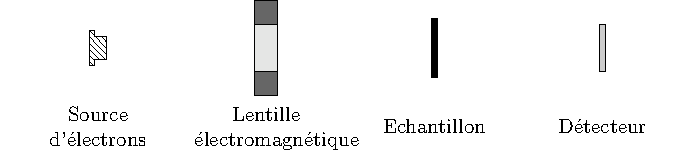
\includegraphics[]{img/chapitre1/figure1/subfig-a/electronic-legend.pdf}
       	}\\
       	\subfigure[Le microscope \gls{tem}]{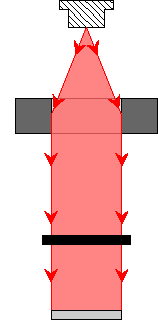
\includegraphics[]{img/chapitre1/figure1/subfig-b/electronic-tem.pdf}}
       	\hspace*{2cm}
       	%
       	\subfigure[Le microscope \gls{stem}]{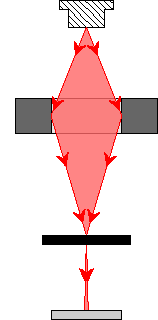
\includegraphics[]{img/chapitre1/figure1/subfig-c/electronic-stem.pdf}}
       	\hspace*{2cm}
       	%
       	\subfigure[Le microscope \gls{sem}]{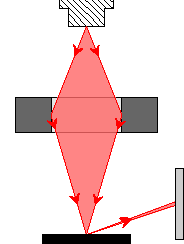
\includegraphics[]{img/chapitre1/figure1/subfig-d/electronic-sem.pdf}}
       	%
           \vspace{1em}
       	\caption{Schéma de principe des différents types de microscopie électronique.%
               \protect\label{fig-chap2-micros-electron}}
   \end{figure*}

    Les microscopes \gls{stem} et \gls{sem} se différencient du \gls{tem} puisque le faisceau balaye l'échantillon ligne par ligne au lieu de l'illuminer entièrement. Il en résulte que ces premiers sont destinés principalement à la \emph{spectroscopie}, \ie{} à l'acquisition d'un spectre pour chaque position spatiale. Les données peuvent alors être représentées comme un cube ayant deux dimensions spatiales et une dimension spectrale. Les applications classiques de ces systèmes sont la détection et cartographie d'éléments chimiques présents dans l'échantillon (\cf{} \cref{sec-exploitation-eels}). Le \gls{tem} est davantage utilisé en \emph{imagerie} pour représenter l'échantillon sans analyse chimique possible.

    La suite de ce manuscrit se focalisera sur la microscopie \gls{stem} qui est le centre de notre étude. C'est pourquoi le principe physique de la microscopie en transmission est évoqué à la \cref{subsec-principe-physique-tem} et les modalités d'acquisition classiques sont présentées à la \cref{subsec-modalitees-stem}. A cette fin, un schéma plus détaillé de ce système et de ses modalités d'acquisition est donné à la \cref{fig-chap2-stem-detail}. Enfin, le contenu technique de ce chapitre s'inspire des livre de Egerton~\cite{egerton2011electron} et de Colliex~\cite{colliex1998microscopie} et nous renvoyons les lecteurs curieux à ces ouvrages pour de plus amples informations.

    \begin{figure*}[htbp]
    	\centering
    	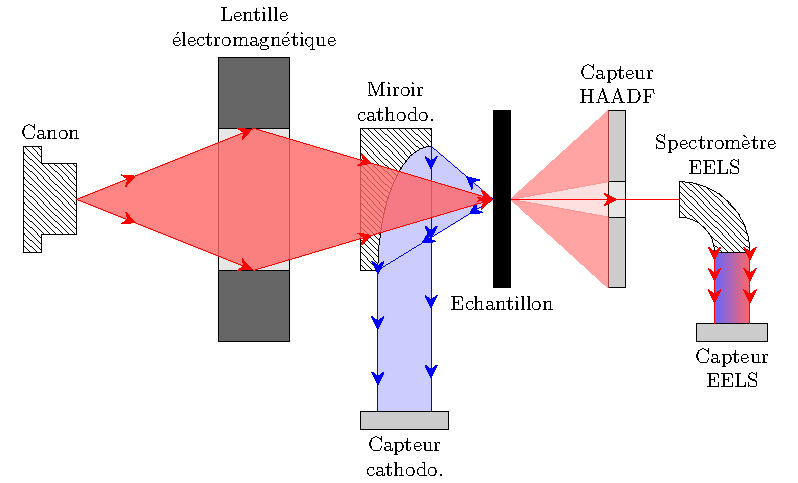
\includegraphics[]{img/chapitre1/figure2/stem-detail.pdf}
    	\caption{Un schéma de principe détaillé du \gls{stem}.
        	\protect\label{fig-chap2-stem-detail}}
    \end{figure*}

    \subsection{Principe de la microscopie en transmission}\label{subsec-principe-physique-tem}

    La microscopie en transmission étudie les interactions physiques entre un faisceau d'électron et la matière qu'il traverse. Pour ce faire, un canon fournit une certaine énergie cinétique à un faisceau d'électrons, celui-ci est alors focalisé en un point de l'échantillon à l'aide de lentilles électromagnétiques. Afin que ce faisceau \emph{traverse} l'échantillon, plusieurs conditions doivent être réunies :
    \begin{enumerate}[label=(\alph*)]
    	\item l'énergie cinétique des électrons doit être suffisante (typiquement 100keV, soit environ 2/3 de la vitesse de la lumière),
    	\item l'échantillon doit être suffisamment fin (typiquement 100nm pour un faisceau de 100keV).
    \end{enumerate}
    Dans ces conditions, les électrons traversent l'échantillon sans subir d'absorption ni de réflexion notoire. A noter qu'il est nécessaire de faire le vide dans le corps du microscope afin d'éviter toute collision entre le faisceau et les molécules d'air. Dès lors, deux types d'interactions électron-atome vont avoir lieu \emph{au sein de l'échantillon}, schématisées aux figures~\ref{fig-chap2-interactions-a} et \ref{fig-chap2-interactions-b}.

    Tout d'abord, l'électron incident interagit avec le noyau de l'atome fortement chargé par une attraction électrostatique d'autant plus intense que celui-ci s'approche du noyau, comme le montre la figure~\ref{fig-chap2-interactions-a}. Cette interaction est appelée diffusion élastique puisqu'il n'y a pas de perte d'énergie cinétique. Cela dit, la majorité des électrons traversent l'atome suffisamment loin du noyau pour être peu déviés et la déviation angulaire associée est de l'ordre du demi-degré (10\;mrad).
    
    D'autre part, l'électron incident traversant le nuage électronique peut interagir avec les électrons le constituant et leur communique de l'énergie, c'est-à-dire dans le modèle atomique les faire passer d'un niveau à un autre ou même les expulser complètement de façon à transformer l'atome initialement neutre en ion. La perte  d'énergie subie par l'électron incident est ainsi gagnée par l'électron de la cible, comme montré sur les figures~\ref{fig-chap2-interactions-b} et \ref{fig-chap2-interactions-c}. Ce type d'interaction mettant en jeu un transfert d'énergie est appelé \emph{diffusion inélastique}. La déviation angulaire est en général sensiblement plus faible que dans le cas de la diffusion élastique et les électrons concernés sont concentrés dans un domaine angulaire restreint (de l'ordre de 0.1 à 1\;mrad).
    
    Pour résumer, les électrons traversant l'échantillon peuvent être déviés de leur trajectoire par diffusion élastique ou inélastique et une partie d'entre eux ont perdu de l'énergie cinétique par diffusion inélastique. Les modalités d'acquisition du \gls{stem} se basent sur la détection de ces deux effets.

    \begin{figure}
    	\centering
    	\subfigure[Diffusion élastique]{
    \begin{tikzpicture}[scale=0.4]
        \clip (-2.6, -5) rectangle (2.5, 5);
        \coordinate (O) at (0, 0);
        \coordinate (A) at (0.4, 4);
        \coordinate (B) at (1.9, 4);

        % Circles
        \draw (O) circle (1cm);
        \draw (O) circle (2cm);

        % Central atom
        \fill[black] (O) circle (0.1cm);

        % Atoms on layers # 1
        \fill[black] (0:1) circle (0.1cm);
        \fill[black] (180:1) circle (0.1cm);

        % Atoms on layers # 2
        \fill[black] (45:2) circle (0.1cm);
        \fill[black] (90+45:2) circle (0.1cm);
        \fill[black] (180+45:2) circle (0.1cm);
        \fill[black] (270+45:2) circle (0.1cm);

        % Incident atoms
        \fill[black] (A) circle (0.1cm);
        \fill[black] (B) circle (0.1cm);

        \draw[->, thick ] (A) -- (0.4, 0) arc (0:-140:0.4) -- ++ (140:3);
        \draw[->, thick, rounded corners=1cm ] (B) -- ++(0, -4.5) -- (-2.5, -3);

    \end{tikzpicture}
    \label{fig-chap2-interactions-a}
}\quad
\subfigure[Diffusion inélastique]{\small
    \begin{tikzpicture}[scale=0.4]
        \clip (-3.25, -5) rectangle (3.25, 5);

        \coordinate (O) at (0, 0);
        \coordinate (A) at (1.4, 4);

        % Circles
        \draw (O) circle (1cm);
        \draw (O) circle (2cm);

        % Central atom
        \fill[black] (O) circle (0.1cm);

        % Atoms on layers # 1
        \fill[black] (0:1) circle (0.1cm);
        \fill[black] (180:1) circle (0.1cm);

        % Atoms on layers # 2
        \filldraw [draw=black, fill=white] (45:2) circle (0.1cm);
        \fill[black] (90+45:2) circle (0.1cm);
        \fill[black] (180+45:2) circle (0.1cm);
        \fill[black] (270+45:2) circle (0.1cm);

        % Layer # 3
        \fill [black!15, even odd rule] (O) circle (3.25cm) circle (2.75cm);
        \draw [densely dashed] (O) circle (3cm);

        % Incident atoms
        \fill[black] (A) circle (0.1cm);
        \draw (A) node [right] {$E_0$};
        \draw[->, thick, rounded corners=1cm ] (A) -- ++(0, -2.55) -- (-1.5, -3.5) node [below] {$E_0-\Delta E$};

        % Other atom and arrows
        \fill [black] (45:3) circle (0.1cm);
        \draw [->, rotate=45] (2.2, 0.1) -- ++ (0.6, 0);
        \draw [<-, dashed, rotate=45] (2.2,- 0.1) -- ++ (0.6, 0);

    \end{tikzpicture}
    \label{fig-chap2-interactions-b}
}\quad
\subfigure[Transition énergétique en diffusion inélastique]{\small
    \begin{tikzpicture}[scale=0.4]
        %\clip (-3.25, -4) rectangle (3.25, 4);

        % horiz. lines
        \draw (0, 1) node [left] {$E_{\text{1s\textsuperscript{2}}}$} -- (5, 1) node [right] {1s\textsuperscript{2}};
        \draw (0, 3) node [left] {$E_{\text{2s\textsuperscript{2}}}$} -- (5, 3) node [right] {2s\textsuperscript{2}};
        \draw (0, 4) node [left] {$E_{\text{2p\textsuperscript{6}}}$} -- (5, 4) node [right] {2p\textsuperscript{6}};

        % Valance band
        \fill [black!15] (0, 6) -- (5, 6) -- (5, 8) -- (0, 8) -- cycle;
        \draw (0, 6) -- (5, 6);
        \draw [thick] (0, 8) node [left] {$E_F$} -- (5, 8);
        \draw (5, 7) node [right] {BV};

        % Left axis
        \draw [->] (0, 0) -- (0, 10) node[above] {$E$};

        % Atoms
        \foreach \n in {1, 1.5}{\fill [black] (\n, 1) circle (0.1cm);}
        \foreach \n in {1, 1.5}{\fill [black] (\n, 3) circle (0.1cm);}
        \foreach \n in {1, 1.5, ..., 3}{\fill [black] (\n, 4) circle (0.1cm);}

        % Moved atom
        \fill [draw=black, fill=white] (3.5, 4) circle (0.1cm);
        \draw [->] (3.5, 4) -- (3.5, 7) node [left] {$\Delta E$};

    \end{tikzpicture}
    \label{fig-chap2-interactions-c}
}

        \vspace{1em}
    	\caption{Une représentation classique de la diffusion électronique inspirée de~\cite{egerton2011electron} et de \cite{colliex1998microscopie}.
        \subref{fig-chap2-interactions-a} Diffusion élastique : l'électron incident est dévié par interaction électrostatique avec le noyau. 
        \subref{fig-chap2-interactions-b} Diffusion inélastique : l'électron incident perd de l'énergie cinétique en faveur d'un électron du nuage atomique.
        \subref{fig-chap2-interactions-c} Représentation des niveaux d'énergie de l'atome. La diffusion inélastique permet à l'un des électrons du nuage électronique de passer dans un état d'énergie supérieur, en bande de valence ou au-delà.  %  
            \protect\label{fig-chap2-interactions}}
    \end{figure}


    \subsection{Les modalités d'acquisition en microscopie \glsentryshort{stem}}\label{subsec-modalitees-stem}

    Le \gls{stem} permet entre autre trois modalités d'acquisition : la cathodoluminescence, l'acquisition fond noir angulaire à grand angle (ou encore \gls{haadf}) et la spectroscopie par perte d'énergie (ou encore \gls{eels}). La \cref{fig-chap2-stem-detail} sert de support pour situer les capteurs correspondant au sein du \gls{stem}.

    \paragraph*{Cathodoluminescence.} Pour certains échantillons, le faisceau incident produit un phénomène de fluorescence dépendant de la nature de l'échantillon et de ses défauts. La technique consistant à acquérir ce signal et à l'étudier s'appelle \emph{la cathodoluminescence}. Le flux lumineux est recueilli à l'aide d'un miroir situé en amont de l'échantillon puis envoyé vers un spectromètre qui procède à l'analyse.

    \paragraph{\gls{haadf}.} Le faisceau incident se situe dans l'axe optique de l'appareil et une grande partie des électrons traversent l'échantillon en demeurant dans cet axe, la diffusion élastique est alors négligeable. Néanmoins, une partie des électrons sont significativement déviés de l'axe optique en sortie.  Un capteur annulaire placé en aval de l'échantillon capte ces électrons et délivre un signal proportionnel. Cette technique appelée \gls{haadf} permet de fournir une image 2D de l'échantillon. Un exemple d'acquisition \gls{haadf} est fourni à la \cref{fig-chap2-haadf-ex}.

    \begin{figure}%[htbp]
    	\centering
    	\subfigure[\label{fig-chap2-haadf-ex-a}Acquisition basse-résolution]%
            {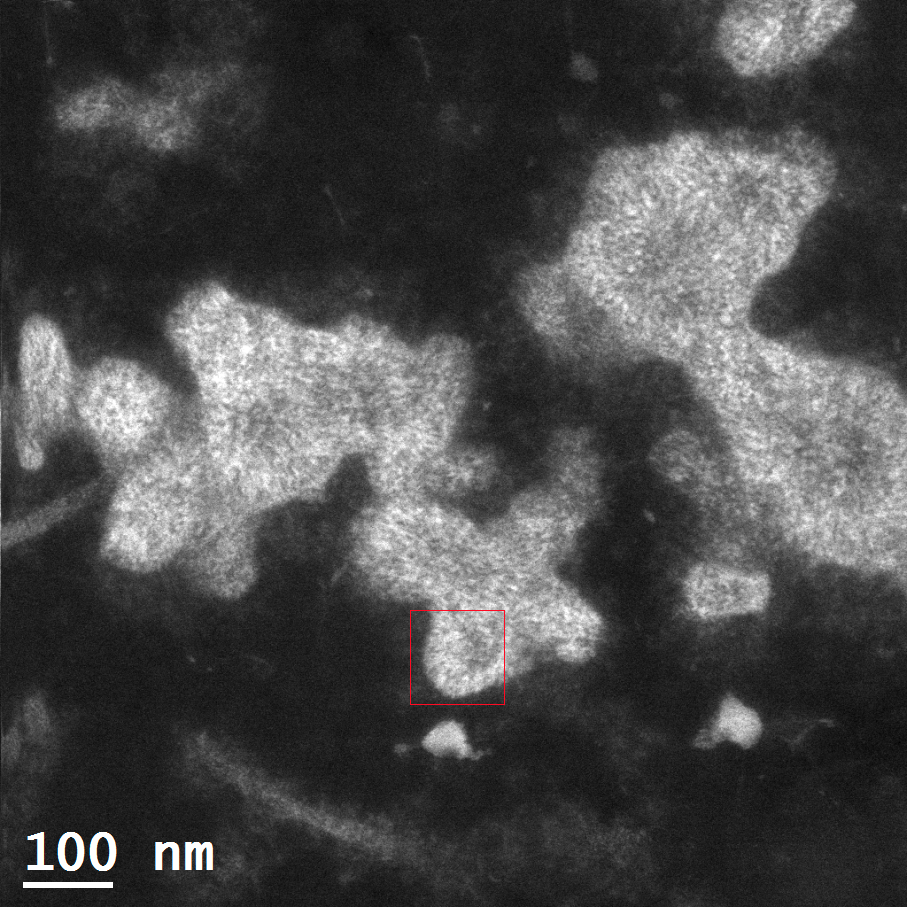
\includegraphics[height=0.25\textwidth]{img/chapitre1/figure4/haadf-LR.png}}
        \hspace{1em}
        \subfigure[\label{fig-chap2-haadf-ex-b}Acquisition haute-résolution]%
            {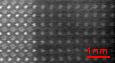
\includegraphics[height=0.25\textwidth]{img/chapitre1/figure4/haadf-HR-sc.png}}
     	%
        \caption{\protect\label{fig-chap2-haadf-ex}Exemples d'acquisitions \gls{haadf}. L'acquisition basse-résolution~\protect\subref{fig-chap2-haadf-ex-a} est de taille micrométrique  tandis que l'acquisition haute-résolution~\protect\subref{fig-chap2-haadf-ex-b} est de taille nanométrique.}
     \end{figure}


    \paragraph*{\gls{eels}.} Comme expliqué précédemment, certains électrons traversant l'échantillon  perdent une partie de leur énergie initiale par diffusion inélastique. Afin de détecter ces pertes, le faisceau demeuré dans l'axe optique frappe un spectromètre séparant les électrons en fonction de leur énergie. Une caméra CCD permet de compter, pour chaque position sur l'échantillon, la quantité d'électrons ayant conservé une énergie donnée. \`A chaque position spatiale correspond alors un spectre de perte d'énergie, les images \gls{eels} sont d'ailleurs également appelées \emph{spectre-image}. La microscopie \gls{eels} constitue le centre de cette étude, c'est pourquoi nous allons détailler ces données et leurs propriétés dans la section suivante.


    \section{Propriétés des données \glsentryshort{eels}}\label{sec-prop-eels}

    \begin{figure}[t]
        \centering
        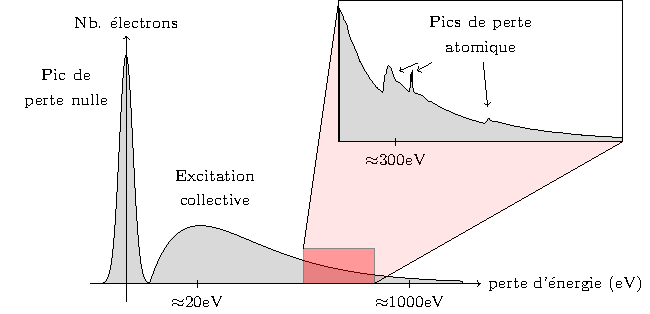
\includegraphics[]{img/chapitre1/figure5/eels-spectrum-shape.pdf}
        \caption{Représentation d'un spectre \gls{eels}.
            \protect\label{fig-chap2-eels-spectrum-shape}}
    \end{figure}

    \subsection{Caractéristiques spectrales} La forme générique d'un spectre \gls{eels} est représentée à la \cref{fig-chap2-eels-spectrum-shape} et affiche le nombre d'électrons ayant traversé l'échantillon en fonction de l'énergie perdue après la traversée (on parle de \emph{canal} pour désigner l'indice associé à une perte d'énergie). Il se compose de trois parties :
    \begin{itemize}
    	\item un pic de perte nulle qui correspond à l'ensemble des électrons ayant traversé l'échantillon sans interagir avec lui, et donc sans avoir perdu d'énergie,
    	\item un pic plus étalé correspondant à une excitation collective de la bande de valence,
    	\item une zone d'intérêt où un ensemble de pics caractéristiques (appelés \emph{seuils}) émergent du fond décroissant.
    \end{itemize}
    \emph{L'information utile est portée par la position, la forme et l'amplitude des seuils}. En effet, la position d'un seuil permet de déterminer l'élément présent dans l'échantillon tandis que son amplitude nous renseigne sur son abondance pour chaque position spatiale. Enfin, la forme du seuil peut varier suivant la configuration électronique de l'élément étudié.
    %
    \`A titre d'exemple, les seuils généralement rencontrés dans nos données se situent à des pertes d'énergie de l'ordre de \np{500} à \np[eV]{1000} (pour rappel, une énergie typique en amont de l'échantillon est \np[keV]{100}).
    %
    Des exemples réels de spectres sont donnés à la \cref{fig-chap2-eels-real-spectra-figure}.


    \begin{normalfigure*}[p]
        \centering
        \subfigure[La position des spectres]{
            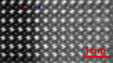
\includegraphics[width=0.3\textwidth]{img/chapitre1/figure6/eels_spectra_haadf-sc.png}
            \label{fig-chapitre2-real-eels-haadf}
        }\\
        \subfigure[Les spectres pour les trois positions]{
            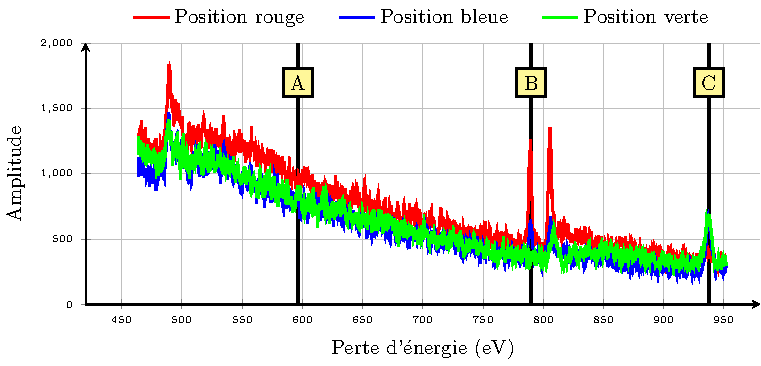
\includegraphics[]{img/chapitre1/figure6/eels_spectra.pdf}
            \label{fig-chapitre2-real-eels-spectra}
        }\\
        %
        \subfigure[Bande A]{% $\mathrm{O-K}$
            
\includegraphics[width=0.3\textwidth]{img/chapitre1/figure6/eels_spectra_band_410.png}
            \label{fig-chapitre2-real-eels-bandA}
        }
        \hspace*{0.5cm}
        %
        \subfigure[Bande B ($\mathrm{La-M}_{4, 5}$)]{
            
\includegraphics[width=0.3\textwidth]{img/chapitre1/figure6/eels_spectra_band_1001.png}
            \label{fig-chapitre2-real-eels-bandB}
        }
        \hspace*{0.5cm}
        %
        \subfigure[Bande C ($\mathrm{Nd-M}_{4, 5}$)]{
            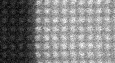
\includegraphics[width=0.3\textwidth]{img/chapitre1/figure6/eels_spectra_band_1465.png}
            \label{fig-chapitre2-real-eels-bandC}
        }

        \caption{Exemple réel de spectre-image \gls{eels}. La figure~\protect\subref{fig-chapitre2-real-eels-haadf} représente l'image \gls{haadf} de l'acquisition et trois positions en rouge, bleu et vert. Les spectres acquis en ces trois positions sont représentés à la figure~\protect\subref{fig-chapitre2-real-eels-spectra}. Enfin, les images à trois niveaux de perte d'énergie (notées A, B et C sur la figure~\subref{fig-chapitre2-real-eels-spectra}) sont représentées aux figures~\subref{fig-chapitre2-real-eels-bandA} à \subref{fig-chapitre2-real-eels-bandC}. Les bandes B et C correspondent respectivement aux signatures $\mathrm{La-M}_{4, 5}$ et $\mathrm{Nd-M}_{4, 5}$ tandis que la bande A ne correspond à aucune signature.
            \protect\label{fig-chap2-eels-real-spectra-figure}}
    \end{normalfigure*}

    \begin{figure*}[]
        \centering
        \subfigure[\label{fig-seuil-a}]{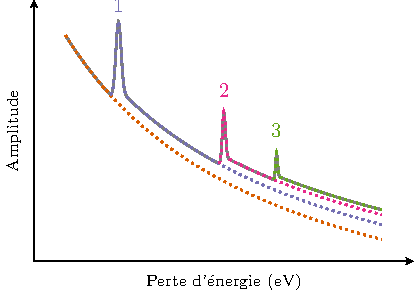
\includegraphics[]{img/chapitre1/figure6-bis/seuils.pdf}}
        \hspace{1em}
        \subfigure[\label{fig-seuil-b}]{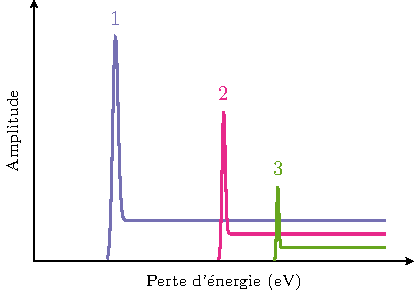
\includegraphics[]{img/chapitre1/figure6-bis/seuils-2.pdf}}
        \caption{Visualisation des effets des seuils successifs sur le spectre. La figure~\subref{fig-seuil-a} représente un spectre constitué de trois seuils. La figure~\subref{fig-seuil-b} représente les effets isolés de chacun des trois seuils. 
            \protect\label{fig-decroissance-spectre}}
    \end{figure*}

    La forme d'un seuil ne se limite pas au seul pic pour des raisons physiques, mais elle se poursuit au-delà puisque l'électron éjecté par diffusion inélastique peut avoir tout un continuum d'énergie au-delà de l'énergie de Fermi. Plus précisément, la forme du seuil varie en fonction des atomes présents au voisinage de l'élément d'intérêt, on parle de \emph{structure fine}.
    
    Le spectre acquis se décompose en un fond continu représentant l'ensemble des contributions des seuils antérieurs et d'autres phénomènes physiques, généralement modélisé par une exponentielle décroissante, et en un ensemble de seuils d'intérêt situés dans la fenêtre d'observation. La \cref{fig-decroissance-spectre} illustre cela. Cette décomposition est à la base des techniques de cartographie que l'on décrira en \cref{sec-exploitation-eels}.
    

    \subsection{Caractéristiques spatiales} En microscopie, comme pour beaucoup de systèmes d'imagerie, la caractéristique principale est le pouvoir séparateur de l'instrument, aussi appelé résolution. En microscopie \gls{stem}, celle-ci est principalement limitée par la taille de la sonde électronique (typiquement 1~nm) et par les aberrations sphériques (un correcteur permet de descendre à 0.1~nm). D'autre part, la résolution, telle qu'entendue en traitement du signal\footnote{La résolution de l'image correspond au nombre de pixels par unité de longueur. Pour éviter toute ambiguïté, on désignera par la suite la résolution de l'instrument par le terme \guillemets{pouvoir séparateur}, plus explicite.}, est choisie par l'expérimentateur en fonction de la distance parcourue par la sonde entre deux acquisitions. Cependant, en imagerie \gls{eels}, la taille de l'image excède rarement $10^5$ pixels pour limiter le temps d'acquisition et éviter de détériorer l'échantillon (comme décrit à la section~\ref{sec-ech-sensibles}). Par conséquent, deux situations apparaissent~:
    \begin{itemize}
        \item l'expérimentateur étudie des structures spatiales étendues (typiquement 100~nm) et est obligé de limiter la résolution, les images sont alors basse-résolution (\cf{} \cref{fig-chap2-haadf-ex-a}),
        \item l'expérimentateur étudie des réseaux atomiques très localisés (typiquement quelques nanomètres) et la résolution est limitée par l'instrument, les images sont alors haute-résolution (\cf{} \cref{fig-chap2-haadf-ex-b}).
    \end{itemize}
    Enfin, il faut noter que la structure spatiale est plus ou moins visible selon le canal considéré dans l'image \gls{eels}. Par exemple, la \cref{fig-chapitre2-real-eels-bandA} correspond à une zone du spectre où aucun contraste n'apparaît clairement, il en résulte que l'image est fortement bruitée. A contrario, les images situées sur des seuils particuliers du spectre sont moins bruitées et mettent clairement en évidence la position des éléments concernés, comme pour les \cref{fig-chapitre2-real-eels-bandB,fig-chapitre2-real-eels-bandC}.  La cartographie des éléments présents dans l'échantillon requiert des méthodes particulières afin de soustraire la contribution du fond continu, comme nous le verrons à la \cref{sec-exploitation-eels}.

    \subsection{Nature du bruit}\label{sec-nature-bruit}
    
    Les sources de bruit sont multiples en imagerie \gls{eels}, mais le type de bruit le plus attendu est poissonien. Cela modélise tant la probabilité qu'un électron du faisceau subisse un certain nombre de diffusions inélastique au sein de l'échantillon~\cite[Section~4.1.1]{egerton2011electron} que la probabilité qu'une cellule du capteur reçoive un électron sur une période donnée. \`A cela s'ajoute un bruit gaussien dû à l'électronique d'acquisition.
    %
    En pratique, la nature du bruit est expérimentalement complexe à déterminer.
    %
    \`A ce bruit d'acquisition vient s'ajouter les instabilités spatiales de l'échantillon : celui-ci dérive au cours de l'acquisition à cause de variations de température et de mouvements d'air~\cite{zobelli2019spatial}. Ces déplacements ne sont pas visibles pour des images basse-résolution mais deviennent critiques à des échelles atomiques puisque le réseau atomique initialement aligné peu apparaître déformé\footnote{Ce n'est pas systématiquement le cas puisque l'expérimentateur limite la dérive, comme expliqué à la section~\ref{sec-ech-sensibles}.}, comme le montre la \cref{fig-drift}.
    %


    \subsection{ACP et redondance spectrale}\label{sec-acp-redondance}

    Le spectre-image \gls{eels} comporte généralement une grande quantité de pixels $\gls{P}\approx 10^4$ et de canaux $\gls{M}\approx 10^3$, conduisant à un nombre de coefficients de l'ordre de $10^7$. La très grande dimension de ces données complique toute analyse directe de l'image et l'on cherche à simplifier l'étude \emph{en réduisant la taille des données tout en conservant le maximum d'information intrinsèque}. Un outil fondamental permettant cela est l'\gls{acp} qui réduit la dimension des données en extrayant les composantes les plus informatives. Cette technique présentée dans cette section s'appuie sur une propriété essentielle des données \gls{eels} : la redondance spectrale.

    \begin{marginfigure}
        \centering
        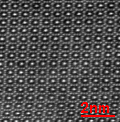
\includegraphics[width=0.7\textwidth]{img/chapitre1/figure7/drift-sc.png}
        \caption{Un exemple de défaut en haute résolution : la dérive de l'échantillon. L'échantillonnage se fait ligne par ligne. On observe que, dans ce cas, l'échantillon dérivait sur la gauche, puis vers le haut. Il en résulte une déformation notable et préjudiciable du réseau atomique.
            \protect\label{fig-drift}}
    \end{marginfigure}

    \paragraph{Présentation générale de l'ACP.} L'\gls{acp} est une technique utilisée en analyse multivariée qui consiste à transformer $M$ variables corrélées entre elles en autant de nouvelles variables décorrélées les unes des autres. Pour cela, la transformation estime successivement les axes dans $\mathbb{R}^M$ maximisant la variance des variables projetées sur cet axe (à chaque nouvel axe estimé, sa contribution est soustraite aux données avant d'estimer l'axe suivant). Ces axes successifs sont appelés les \emph{composantes principales des données}.
    Plus précisément, cette transformation décrite plus en détail dans~\cite{jolliffe2002springer} requiert le spectre-image \gls{Y} de taille \taille{M}{P} où chaque colonne correspond à un spectre \gls{eels} et où chaque ligne est une image pour un canal donné. Notons que la moyenne empirique des spectres est supposée être soustraite de sorte que les données $\tilde{\mathbf{Y}}=\gls{Y}-\frac{1}{P}\sum_p\mathbf{Y}_p$ soient centrées.
    %
    Ainsi, l'ACP transforme l'image $\tilde{\gls{Y}}$ dont les spectres sont possiblement corrélés en les données transformées $\mathbf{S} = [\mathbf{s}_1,\dots,\mathbf{s}_M]^T$ (aussi appelées \emph{variables de représentation}) décorrélées de telle sorte que
    \begin{equation}\label{eq-decomposition-acp}
    \mathbf{S}_\mathbf{Y} = \gls{H}^T\tilde{\gls{Y}}
    \end{equation}
    où $\gls{H} = [\mathbf{h}_1,\dots,\mathbf{h}_M]$ est une matrice orthogonale de taille \taille{M}{M} contenant les composantes principales de \gls{Y}. Remarquons que l'orthogonalité de \gls{H} dans la transformation~\eqref{eq-decomposition-acp} permet de considérer l'\gls{acp} comme un changement de base dans $\mathbb{R}^M$ dont les vecteurs $\mathbf{h}_1,\dots,\mathbf{h}_M$ forment la nouvelle base. 
    %
    En pratique, la matrice $\gls{H}$ est obtenue en diagonalisant la matrice de variance-covariance $\tilde{\mathbf{C}} = \frac{1}{p-1}\tilde{\gls{Y}}\tilde{\gls{Y}}^T$. Les vecteurs propres constituent la matrice $\gls{H}$ tandis que chaque valeur propre $\gls{d}_m$ correspond à la variance de la représentation $\mathbf{s}_m$ pour une composante principale $\mathbf{h}_m$ donnée. On désigne ainsi la valeur propre $\gls{d}_m$ comme la puissance associée à la composante principale $\mathbf{h}_m$ et les colonnes de \gls{H} sont triées par puissance décroissante. 
    %
    Enfin, précisons que l'estimation des composantes principales est d'autant meilleure que la matrice de covariance est correctement estimée, à savoir $P\gg M$.

    \paragraph{Matrice de covariance ou matrice de corrélation ?} Dans le paragraphe précédent, la moyenne empirique $\boldsymbol\mu = [\mu_1,\dots,\mu_M]^T$ a été soustraite aux données afin d'obtenir les données centrées
    \begin{equation}
     \tilde{\mathbf{Y}} =
        \begin{pmatrix}
        \mathbf{Y}_{1 1} - \mu_1&\mathbf{Y}_{1 2} - \mu_1&\cdots&\mathbf{Y}_{1 P} - \mu_1\\
        \mathbf{Y}_{2 1} - \mu_2&\mathbf{Y}_{2 2} - \mu_2&\cdots&\mathbf{Y}_{2 P} - \mu_2\\
        \vdots&\vdots&\ddots&\vdots\\
        \mathbf{Y}_{M 1} - \mu_M&\mathbf{Y}_{M 2} - \mu_M&\cdots&\mathbf{Y}_{M P} - \mu_M
        \end{pmatrix}.
    \end{equation}
    La matrice de covariance $\tilde{\mathbf{C}} = \frac{1}{p-1}\tilde{\gls{Y}}\tilde{\gls{Y}}^T$ est ensuite calculée afin d'extraire les composantes principales. Cette méthode a un défaut majeur : si un canal d'indice $m_0\in\llbracket 1,M\rrbracket$ correspond à un seuil d'amplitude très supérieure aux amplitudes des autres seuils, alors celui-ci va \guillemets{tirer} les résultats de l'ACP vers lui au détriment des autres caractéristiques~\cite[Section~3.3]{jolliffe2002springer}.
    %
    Dans ce genre de cas, l'alternative consiste estimer les écarts-types empiriques $\boldsymbol\sigma=[\sigma_1,\dots,\sigma_M]^T$, puis à réduire les données
    \begin{equation}
    \bar{\mathbf{Y}} =
    \begin{pmatrix}
    \frac{\mathbf{Y}_{1 1} - \mu_1}{\sigma_1}&
    \frac{\mathbf{Y}_{1 2} - \mu_1}{\sigma_1}&
    \cdots&
    \frac{\mathbf{Y}_{1 P} - \mu_1}{\sigma_1}\\
    %
    \frac{\mathbf{Y}_{2 1} - \mu_2}{\sigma_2}&
    \frac{\mathbf{Y}_{2 2} - \mu_2}{\sigma_2}&
    \cdots&
    \frac{\mathbf{Y}_{2 P} - \mu_2}{\sigma_2}\\
    %
    \vdots&\vdots&\ddots&\vdots\\
    %
    \frac{\mathbf{Y}_{M 1} - \mu_M}{\sigma_M}&
    \frac{\mathbf{Y}_{M 2} - \mu_M}{\sigma_M}&
    \cdots&
    \frac{\mathbf{Y}_{M P} - \mu_M}{\sigma_M}
    \end{pmatrix}.
    \end{equation}
    La matrice de \emph{corrélation} $\bar{\mathbf{C}} = \frac{1}{p-1}\bar{\gls{Y}}\bar{\gls{Y}}^T$ est ensuite diagonalisée afin d'extraire les composantes principales. %
    %
    Si cette technique permet de prévenir le défaut lié à la matrice de covariance, elle présente elle-même un inconvénient puisqu'elle est plus apte à capturer des seuils apparentés au bruit.
    %
    Ces aspects sont détaillés et discutés a l'annexe~\ref{abstr-pca-corr-cov}. Dans le cadre de cette étude, la matrice de covariance sera utilisée.


    \paragraph{L'ACP en vue de réduire la dimension.} L'ACP est d'autant plus performante à réduire la dimension des données que celles-ci sont corrélées. En effet, si les observations sont fortement corrélées, on observe que les variances des variables de représentation associées aux premières composantes principales sont particulièrement élevées par rapport aux variances des variables de représentation associées aux dernières composantes principales.
    %
    Ainsi, l'on observe généralement un changement de comportement à un indice $\gls{R}\ll M$ d'autant plus faible que les données sont corrélées, ou à défaut de variation brutale de la courbe des puissances, on choisit l'indice \gls{R} tel que les \gls{R} premières composantes principales regroupent une fraction élevée de la puissance totale.
    %
    Dans ce cas, il est possible d'approximer les données \gls{Y} par une matrice $\hat{\gls{Y}}_{1:R}$ en projetant les données sur le sous-espace de dimension \gls{R} généré par les \gls{R} premières composantes principales, puis en les rétro-projetant dans $\mathbb{R}^M$. Ainsi, l'approximation à l'ordre \gls{R} s'écrit
    \begin{equation}
    \hat{\gls{Y}}_{1:R} = \gls{H}_{1:R}\gls{H}_{1:R}^T\gls{Y}
    \end{equation}
    où $\gls{H}_{1:R}$ correspond aux $R$ premières colonnes de $\gls{H}$. Cette approximation est d'autant plus fidèle que les données sont fortement corrélées, comme le montre la \cref{fig-pca-data-corr}.

    \begin{figure*}[]
        \centering
        \subfigure[\label{fig-pca-data-corr-a}$\mathrm{corr} = 0$]{
            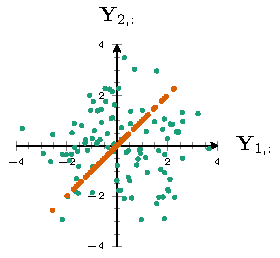
\includegraphics{img/chapitre1/figure15/pca-corr-1.pdf}}
        \subfigure[\label{fig-pca-data-corr-b}$\mathrm{corr} = 0.95$]{
            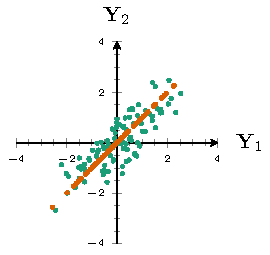
\includegraphics{img/chapitre1/figure15/pca-corr-2.pdf}}
        \subfigure[\label{fig-pca-data-corr-c}$\mathrm{corr} = 99$]{
            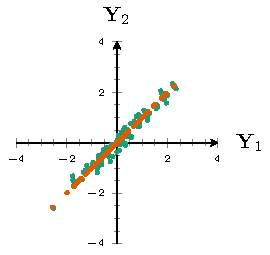
\includegraphics{img/chapitre1/figure15/pca-corr-3.pdf}}
        \caption{Trois exemples de nuages de points avec $M=2$ et $P=100$ (en vert) et leur approximation au 1er ordre (en orange). Les coefficients de corrélation valent respectivement 0, 0.95 et 0.99 pour les figures~\protect\subref{fig-pca-data-corr-a}, \protect\subref{fig-pca-data-corr-b} et \protect\subref{fig-pca-data-corr-c}. L'approximation du premier ordre est d'autant meilleure que les données sont corrélées. En particulier, ne conserver que la première composante principale est suffisant pour la figure~\protect\subref{fig-pca-data-corr-c}.
            \protect\label{fig-pca-data-corr}}
    \end{figure*}

    \paragraph{Application aux données EELS.} L’imagerie hyperspectrale est une technique combinant l’imagerie et la spectroscopie où chaque pixel de l'image est caractérisé par un spectre électromagnétique. Ces images spectroscopiques sont utilisés dans de nombreux domaines incluant la télédétection~\cite{schaepman2009earth}, la planétologie~\cite{smith1985quantitative}, le contrôle des aliments~\cite{gowen2007hyperspectral} et l'ingénierie biomédicale~\cite{akbari2010detection}. Si les spectres \gls{eels} ne sont pas de nature électromagnétiques, les spectre-images sont néanmoins un cas particulier d'images hyperspectrales puisqu'elles partagent un très grand nombre de propriétés et de méthodes d'analyse.
    %
    La popularité de ces techniques découle d'une propriété fondamentale des données hyperspectrales~: la redondance spectrale. En effet, les spectres issus de ces images sont connus pour être fortement corrélés spectralement~\cite{dobigeon2016linear, bioucas2012hyperspectral, dobigeon2012spectral} et le paradigme du démélange (discuté en détail à la \cref{sec-demelange}) en donne une interprétation physique. Dans ce paradigme, chaque spectre acquis est supposé être le mélange de signatures spectrales élémentaires appelés \emph{endmembers} correspondant à des éléments particuliers de la scène (\eg{} de l'eau, des bâtiments ou de la végétation en télédétection).
    %
    Tout cela permet de conclure que les spectres, loin de remplir $\mathbb{R}^M$ uniformément, évoluent dans une variété de dimension $\gls{R}\ll M$. Par défaut, cette variété n'est pas plane puisque des non-linéarités interviennent dans le mélange, causés par des phénomènes physiques au niveau local. Néanmoins, une approximation linéaire peut être réalisée afin d'estimer le sous-espace de dimension réduite appelé \emph{sous-espace signal}, possiblement à l'aide d'une \gls{acp}. L'identification de ce sous-espace permet d'obtenir des variables de représentation de dimension réduite pourtant très précises, ouvrant la voie à un gain considérable en temps de calcul, en complexité et en stockage de donnée pour une qualité d'image équivalente. Comme expliqué plus haut, l'\gls{acp} réduit d'autant la dimension du spectre-image (ou encore \gls{R} est d'autant plus faible) que les données sont corrélées \ie{} que peu d'éléments élémentaires sont présent dans la scène. La \cref{fig-ACP} montre les composantes principales d'un spectre-image réel. L'évolution des puissances issues de l'\gls{acp} affichées à la \cref{fig-sub-pca-eigs} nous permet de déterminer trois comportements\footnote{Il faut noter que les puissances ont été corrigées afin de compenser l'erreur d'estimation dû au faible nombre d'observations (le nombre de pixels est du même ordre de grandeur que le nombre de canaux), comme expliqué à la \cref{subsec-3s-acp}.}.
    \begin{normalfigure*}[htbp]
        \centering
        \subfigure[Evolution des valeurs propres associées à l'\gls{acp}]{
            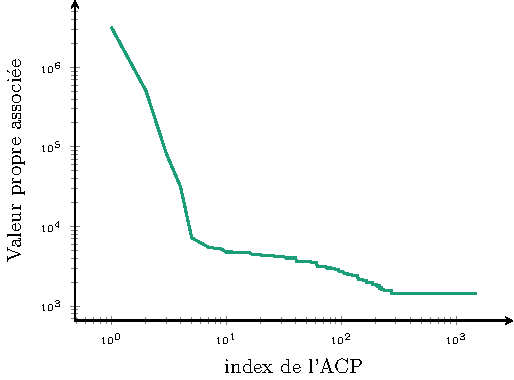
\includegraphics[]{img/chapitre1/figure9/PCA_eigs.pdf}
            \label{fig-sub-pca-eigs}}
        \\
        \subfigure[Variable de repr. \num\ 1]{\label{fig-sub-pca-comp1}
            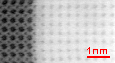
\includegraphics[width=0.28\textwidth]{img/chapitre1/figure9/PCA_map_0-sc.png}}\vspace{20pt}
        \subfigure[Variable de repr. \num\ 2]{\label{fig-sub-pca-comp2}
            
\includegraphics[width=0.28\textwidth]{img/chapitre1/figure9/PCA_map_1.png}}\vspace{20pt}
        \subfigure[Variable de repr. \num\ 3]{\label{fig-sub-pca-comp3}
            
\includegraphics[width=0.28\textwidth]{img/chapitre1/figure9/PCA_map_2.png}}\\
        \subfigure[Variable de repr. \num\ 4]{\label{fig-sub-pca-comp4}
            
\includegraphics[width=0.28\textwidth]{img/chapitre1/figure9/PCA_map_3.png}}\vspace{20pt}
        \subfigure[Variable de repr. \num\ 5]{\label{fig-sub-pca-comp5}
            
\includegraphics[width=0.28\textwidth]{img/chapitre1/figure9/PCA_map_4.png}}\vspace{20pt}
        \subfigure[Variable de repr. \num\ 6]{\label{fig-sub-pca-comp6}
            
\includegraphics[width=0.28\textwidth]{img/chapitre1/figure9/PCA_map_5.png}
        }\\
        %
        \def\comp{mean}
        \subfigure[Spectre moyen]{
            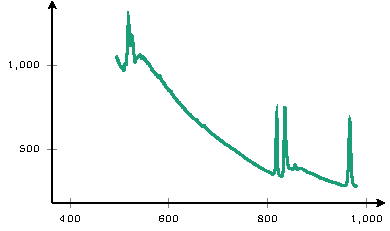
\includegraphics[]{img/chapitre1/figure9/PCA_spectra_1.pdf}
            \label{fig-sub-pca-mean}}%
        %
        \def\comp{comp0}%
        \subfigure[Première composante]{
            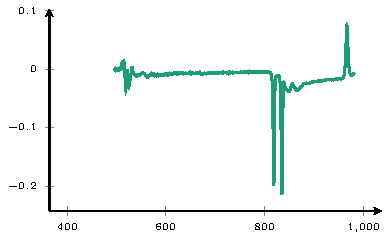
\includegraphics[]{img/chapitre1/figure9/PCA_spectra_2.pdf}
            \label{fig-sub-pca-spectrum-0}}
        %
        \caption{L'analyse par \gls{acp} de données \gls{eels}. La figure~\subref{fig-sub-pca-eigs} représente l'évolution des valeurs propres associées à l'\gls{acp}. On observe, entre autres, que seules les 5 premières composantes sont vraiment significatives. Les figures \subref{fig-sub-pca-comp1} à \subref{fig-sub-pca-comp6} représentent les variables de représentation associées aux composantes principales les plus puissantes. Le spectre moyen donné à la figure~\subref{fig-sub-pca-mean} est soustrait aux données avant d'appliquer l'\gls{acp}. Il en résulte que les spectres associés aux composantes principales sont des variations par rapport à ce spectre moyen, ce qui explique que la première composante affichée à la figure~\subref{fig-sub-pca-spectrum-0} soit parfois négative.
            \protect\label{fig-ACP}}
    \end{normalfigure*}    
    \begin{itemize}
        \item Les premières composantes de puissance très élevées correspondent à des éléments chimiques présents en forte quantité dont les projections associées (\cf{} \crefrange{fig-sub-pca-comp1}{fig-sub-pca-comp4}) renferment beaucoup d'information spatiale et peu de bruit. Le spectre associé à la première composante est lui-même très peu bruité (\cf{} \cref{fig-sub-pca-spectrum-0}).
        \item Un ensemble de composantes principales situées entre les indices 5 et 300 se démarque encore par sa puissance, bien que moins important que les premières composantes. L'évolution de leur puissance est également moins rapide. Il s'agit généralement de composants très localisés spatialement ou issus de mélanges non-linéaires. Certaines informations spatiales peuvent être encore discernées chez les projections associées aux composantes les plus puissantes, comme à la \cref{fig-sub-pca-comp5}.
        \item Les dernières composantes présentent enfin une puissance constante correspondant à la puissance estimée du bruit. Plus aucune information n'est visible ni dans le spectre associé ni dans la projection correspondante.
    \end{itemize}
    Cette observation permet généralement le débruitage des données en supprimant les composantes principales associées au bruit, comme décrit à la \cref{sec-ech-sensibles}. Malheureusement, le choix du seuil \gls{R} correspondant à la dimension du sous-espace estimé n'est pas trivial. Deux solutions seront cependant proposées: l'une basée sur l'évolution des valeurs propres à la \cref{subsec-3s-acp}, l'autre analysant le contenu spatial des images issues des projections sur les composantes principales à l'annexe~\ref{sec-spim-creation-hr}

    

    %
    \section{Cartographie par séparation de composantes spectrales}\label{sec-exploitation-eels}

    Le problème généralement rencontré lors de l'exploitation des données \gls{eels} consiste à localiser et à cartographier un ensemble de composés chimiques élémentaires présents dans l'échantillon~\cite{colliex2012stem, pennycook2011seeing, dobigeon2012spectral}.
    %
    Pour cela, nous pouvons exploiter l'information spectrale contenue aux abords du seuil associé à l'élément étudié. En effet, plus il est abondant en une position spatiale, plus l'amplitude du seuil associé est grande. En couplant l'information obtenue en chaque position, une image appelée \emph{carte d'abondance} renseignant sur sa répartition spatiale peut être générée. 
    %
    Ce problème est plus largement rencontré en imagerie hyperspectrale, comme en télédétection afin de cartographier des constituants élémentaires au sein d'une scène~\cite{lelong1998hyperspectral} (\eg{} eau, bâtiments, etc).
    %
    La technique historique classiquement utilisée en imagerie \gls{eels} analyse de manière supervisée les spectres pris indépendamment afin de quantifier un élément particulier.
    %
    A l'inverse, des approches plus récentes analysent le spectre-image dans son entièreté de manière non-supervisée afin de cartographier l'ensemble des composantes d'intérêt. 


    \subsection{Quantification par ajustement d'exponentielle}
    
    Comme expliqué à la \cref{sec-prop-eels}, un spectre \gls{eels} contient la contribution de plusieurs seuils successifs et d'un fond continu. Pour pallier ce problème, le fond décroissant et la rémanence des seuils précédents devront être soustraits avant d'intégrer le seuil d'intérêt. Pour illustrer cette méthode, considérons le spectre affiché à la \cref{fig-carto-separation-a}, correspondant à une position spatiale donnée. Une zone de régression est choisie en amont du seuil (tout en restant proche du seuil) et une régression exponentielle de la forme $y=Ax^{-r}$ est effectuée (\cf{}~\cite[Section~4.4]{egerton2011electron} pour plus de détails). La courbe estimée est alors soustraite pour obtenir un spectre corrigé propre à ce seuil, \ie{}, le seuil étudié n'est plus influencé par le fond continu. L'abondance du composé pour cette position spatiale est ensuite calculée en sommant le spectre dans une zone centrée sur le seuil d'intérêt. En effectuant cette opération pour toutes les positions spatiales, nous pouvons reconstituer la carte d'abondance de la \cref{fig-carto-separation-b}. \`A noter que les paramètres de la régression dépendent de la position spatiale.

    Afin d'effectuer la cartographie de plusieurs composantes présentes dans l'échantillon, l'expérimentateur doit alors exécuter cette opération pour tous les seuils présents dans le spectre. Cette technique est simple et une implémentation automatique est facile à mettre en \oe{}uvre dès lors que les zones de régression et d'intégration ont été définies.
    
    \begin{figure*}[t]
        \centering
        \subfigure[\label{fig-carto-separation-a}]{
            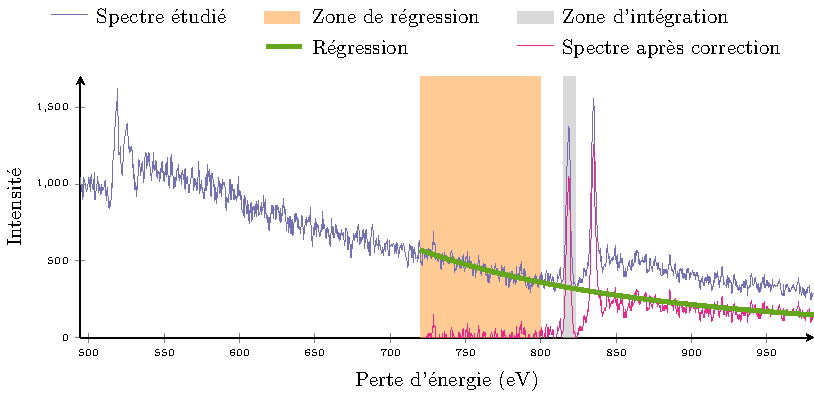
\includegraphics[]{img/chapitre1/figure11/separation.pdf}}\hspace{1em}
        \subfigure[\label{fig-carto-separation-b}]{
            
\includegraphics[width=5cm]{img/chapitre1/figure11/regression-sc.png}}
        \caption{Illustration de la méthode de cartographie par ajustement d'exponentielles spectrales. \protect\subref{fig-carto-separation-a} Régression pour une position particulière. Une régression exponentielle est effectuée sur la zone de régression, puis est soustraite au spectre pour obtenir le spectre corrigé. L'abondance est finalement calculée en intégrant le spectre autours du pic d'intérêt. \protect\subref{fig-carto-separation-b} Résultat en effectuant cette action sur tous les pixels (l'élément cartographié est $\mathrm{La-M}_{4, 5}$). A noter que les paramètres de la régression dépendent de la position spatiale.
            \protect\label{fig-carto-separation}}
    \end{figure*}
    
    Cependant, cette technique ne permet que la \emph{quantification} de l'élément à une constante près quel que soit son environnement\,; elle ne permet entre autres pas d'obtenir des proportions contrairement au démélange discuté à la section suivante. Or, la structure fine, c'est-à-dire la forme du seuil, renseigne sur l'état du composé étudié et la technique ci-dessus ne fait aucune distinction lors de la quantification. Par exemple, les travaux menés dans~\cite{dobigeon2012spectral} s'intéressent à l'état d'oxydation du bore et tentent de cartographier deux états distincts, la forme oxydée B\textsubscript{2}O\textsubscript{3} et la forme azotée BN. Dans ce cas, la technique proposée ne fait pas cette distinction.
    %
    Pour résoudre cette impasse, des techniques de cartographie non-supervisée ont été proposées ces dernières décennies afin de ne pas considérer le pic uniquement, mais l'ensemble du spectre.

    

    \subsection{Techniques de cartographie non-supervisée}\label{sec-demelange}
    
    \paragraph{Approches par ACP et ACI.} La redondance spectrale présentée à la section précédente suggère que les spectres acquis soient le résultat d'un mélange de $N_c$ spectres élémentaires $\mathbf{m}_1,\dots,\mathbf{m}_{N_c}$ appelés \emph{endmember}, correspondant aux signatures associées aux composés caractéristiques présents dans l'échantillon.
    %    
    Estimer les signatures $\mathbf{m}_k$ s'apparente à de la séparation aveugle de sources et les premières techniques non-supervisée proposées l'ont considéré d'un point de vue statistique en usant des techniques d'analyse multivariée. Dans cette perspective, l'\gls{acp} a été utilisée afin d'extraire les signatures de spectre-images \gls{eels} dans~\cite{bonnet1999extracting, bosman2006mapping, trebbia1990eels}, mais cette méthode renvoie des spectres difficiles à interpréter physiquement, à cause notamment de la contrainte d'orthogonalité inhérente à l'\gls{acp} imposée aux endmembers. L'\gls{aci} a été envisagée comme alternative afin d'analyser les données hyperspectrales issues de la télédétection~\cite{bayliss1998analyzing, chen1999independent} ou de l'imagerie \gls{stem}-\gls{eels}~\cite{delapena2011mapping, bonnet2005independent, bosman2006mapping}. Malheureusement, l'\gls{aci} repose sur l'hypothèse que les signatures spectrales comme leur abondance soient indépendantes, ce qui n'est pas le cas puisque si un élément est fortement présent, les autres le seront généralement moins. Cela compromet l'utilisation de l'\gls{aci} en démélange hyperspectral, d'autant que ni l'\gls{acp}, ni l'\gls{aci} ne permettent de contraindre l'abondance à être positive et leurs résultats demeurent en général difficile à interpréter d'un point de vue physique. Toutefois, l'ACI peut donner des résultats intéressants et rapides pour certains jeux de données et cela peut être un point de départ dans l'analyse de l'image.
    
    \paragraph{Approches par démélange.} Comme expliqué précédemment, les spectres acquis sont supposés être le résultat d'un mélange de $N_c$ spectres élémentaires\,; une hypothèse de mélange linéaire est souvent réalisée afin de simplifier l'interprétation et la résolution du problème inverse associé. Dans ce cas, le modèle direct s'écrit~\cite{dobigeon2016linear}
    \begin{align}
    &\gls{Y} = \mathbf{M}\mathbf{A}\\
    \text{tel que}\quad &\mathbf{A} \geq 0\qquad \mathbf{M} \geq 0\label{eq-positivity}\\
    &\sum_k \mathbf{A}_{kp} = 1 \quad \forall p\in\llbracket 1 , P \rrbracket \label{eq-sum-to-one}
    \end{align}
    où $\mathbf{M}=[\mathbf{m}_1,\dots,\mathbf{m}_{N_c}]$ de taille $M\times N_c$ est la matrice contenant les signatures spectrales et où $\mathbf{A} = [\mathbf{a}_1,\dots,\mathbf{a}_{N_c}]^T$ est la matrice d'abondance de taille $N_c\times P$. Chaque ligne $\mathbf{a}_c$ est une image représentant la proportion de l'endmember $\mathbf{m}_k$ au sein de l'échantillon, il s'agit de la carte d'abondance. Deux hypothèses portant sur $\mathbf{A}$ sont réalisées : l'hypothèse de positivité à l'équation~\eqref{eq-positivity} et l'hypothèse de somme à un à l'équation~\eqref{eq-sum-to-one}.
    \begin{description}
        \item[Positivité] L'abondance de l'élément ne peut être négative puisqu'il s'agit d'une proportion. Et puisque le spectre est positif, les entrées de $\mathbf{A}$ et de $\mathbf{M}$ sont donc positives.
        \item[Somme à un] La somme des abondances vaut un pour toute position spatiale. Cette hypothèse traduit le fait que les éléments de $\mathbf{A}$ soient des proportions. Cependant, pour que l'on puisse comparer les proportions d'un pixel à l'autre, il est nécessaire que la quantité de matière traversée par le faisceau soit la même sur l'ensemble de l'échantillon, sans quoi deux proportions identiques ne traduiraient pas une quantité égale de l'élément.
    \end{description}
    Une représentation géométrique du mélange linéaire est donné à la \cref{fig-melange-lineaire} pour $M=3$ et $N_c=3$. Les coordonnées des trois endmembers $\mathbf{m}_1,\mathbf{m}_2,\mathbf{m}_3$ sont représentés dans $\mathbb{R}_3$ et puisque la contrainte de somme à un est utilisée ici, l'ensemble des spectres obtenus par mélange linéaire se situent dans le plan de dimension $M-1=2$ généré par ces trois vecteurs (à condition qu'ils soient linéairement indépendants). Enfin, l'hypothèse de positivité contraint l'ensemble des spectres de \gls{Y} à évoluer dans le simplexe formé par $\mathbf{m}_1$, $\mathbf{m}_2$ et $\mathbf{m}_3$.
    \begin{figure}
        \centering
        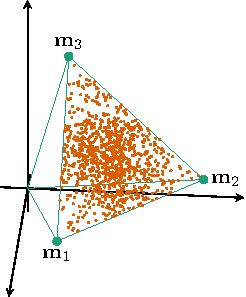
\includegraphics[]{img/chapitre1/figure17/melange_lineaire.pdf}
        \caption{Une représentation géométrique du modèle de mélange linéaire pour $M=3$ et $N_c=3$. Les spectres élémentaires sont notés $\mathbf{m}_1$, $\mathbf{m}_2$ et $\mathbf{m}_3$. La contrainte de somme à un contraint les spectres constitutifs de \gls{Y} (en orange) à évoluer dans le plan formé par ces trois vecteurs tandis que la contrainte de positivité les contraint à demeurer dans le simplexe formé par les endmembers.
            \protect\label{fig-melange-lineaire}}
    \end{figure}
    Maintenant que le modèle direct est posé, le problème inverse consiste à estimer conjointement les spectres élémentaires $(\mathbf{m}_k)_{k=1,\dots,N_c}$ ainsi que les cartes d'abondance associées. Ce problème inverse est appelé \emph{démélange hyperspectral}~\cite{bioucas2012hyperspectral, dobigeon2016linear} ou \emph{unmixing} et s'apparente à un problème de séparation aveugle de source~\cite{comon2010handbook}. Il requiert la connaissance du nombre de composantes $N_c$.
    %
    Une technique de démélange non-supervisée a pour but d'estimer les endmembers, ou de manière géométrique le simplexe dans lequel évoluent les spectres acquis et dont les endmembers constituent les sommets, et la matrice d'abondance associée\footnote{Le nombre d'endmember est lui-aussi inconnu dans la plupart des situations, mais il peut être estimé par une autre méthode a priori.}. Souvent, ce problème d'estimation est généralement non-convexe et on lui préfère une résolution sous-optimale en deux temps. D'abord, les signatures élémentaires sont déterminées à l'aide d'un algorithme d'extraction d'endmember, puis la matrice d'abondance est déterminée. Néanmoins, des méthodes bayésiennes permettent une estimation conjointe des endmembers et de des abondances basées sur un modèle statistique.

    \paragraph{Estimation des endmembers.} Les premières méthodes d'extraction d'endmember utilisées furent l'ACP et l'ACI avec les inconvénients relevés plus haut.
    % 
    Une autre approche du problème consiste à user de l'interprétation géométrique réalisée plus haut afin d'estimer les endmembers $\mathbf{m}_k$. Dans l'hypothèse où les composantes pures sont présentes dans l'échantillon, des techniques efficaces et rapides permettent de déterminer les spectres acquis correspondant aux endmembers. Par exemple, \gls{vca}~\cite{nascimento2005vertex} projette itérativement les données sur un axe orthogonal au sous-espace généré par les endmembers déjà déterminés. Le nouvel endmember correspond au point extrême de la projection et l'algorithme est itéré jusqu'à obtenir toutes les composantes. Néanmoins, l'hypothèse de pixels purs est généralement trop forte. En microscopie \gls{stem}-\gls{eels}, par exemple, à cause d'une résolution insuffisante ou d'une épaisseur d'échantillon permettant la superposition d'éléments différents, on n'acquiert pas de spectre pur. Pour relâcher cette contrainte, les techniques par minimisation de volume estiment la matrice $\mathbf{M}$ de sorte que le simplexe généré par les endmembers $\mathbf{m}_i$ soit de volume minimal tout en contenant l'ensemble des spectres acquis. Ce problème devient plus difficile à résoudre puisqu'il est non-convexe, c'est pourquoi il est initialisé à l'aide d'une autre technique comme \gls{vca}. L'algorithme \gls{sisal}~\cite{bioucas2009variable} implémente une version plus robuste en autorisant la violation de la contrainte de positivité, c'est pourquoi certains spectres estimés par SISAL peuvent être négatifs, mais cette violation est contrainte à l'aide de la fonction hinge $h$ ($h(x) = 0$ si $x \geq 0$ et $h(x)=-x$ si $x<0$). Les techniques par approche géométrique sont rapides et efficaces si l'image présente des pixels purs, autrement, ces performances sont réduites et des techniques statistiques sont à préférer.
    
    \paragraph{Estimation des abondances.} Une fois l'extraction des endmembers réalisée, on doit estimer les abondances.  Cela consiste à déterminer le sous-ensemble optimal de signatures spectrales ainsi que les proportions associées pouvant décrire chaque pixel mélangé de l'échantillon. En pratique, il s'agit d'une régression parcimonieuse linéaire faisant appel à des régularisations parcimonieuses telles que décrites à la \cref{sec-MC-regul}, puisque le nombre de signatures spectrales utilisées pour décrire chaque pixel est supposé être faible devant $N_c$. Un représentant de cette famille de méthodes est \gls{sunsal}~\cite{bioucas2010alternating} qui propose de contraindre la parcimonie des abondances à l'aide d'une norme $\ell_1$ et de résoudre le problème d'optimisation par l'algorithme ADMM~\cite{eckstein1992douglas, combettes2011proximal}.
    
    \paragraph{Estimation conjointe par méthode bayésienne.} D'autres techniques statistiques plus performantes ont également été étudiées, comme les approches bayésiennes qui résolvent les inconvénients de l'ACP et de l'ACI en introduisant des informations a priori, contraignant par là même les solutions à avoir un sens physique. Ces méthodes permettent l'estimation conjointe des endmembers et des abondances. L'algorithme Bayesian linear unmixing (BLU)~\cite{dobigeon2009joint} qui en est un exemple a été appliqué avec succès en imagerie \gls{stem}-\gls{eels}~\cite{dobigeon2012spectral}.
    
    
    %
    \section{L'acquisition d'échantillons sensibles : problématiques et stratégies}\label{sec-ech-sensibles}

    \paragraph{Problématique des échantillons sensibles.} Une problématique récurrente en microscopie est la détection de structures fines dont le seuil associé est de faible amplitude. Dans une telle situation, le \gls{snr} du spectre-image acquis doit être supérieur à un \gls{snr} minimum, nécessaire à la détection précise des structures fines. A cette fin, l'expérimentateur doit augmenter la dose totale d'électrons délivrée à chaque position de l'échantillon. Pour cela, il peut agir sur l'intensité du faisceau ou sur la durée d'exposition par position spatiale (appelé \emph{dwell time}). Quelle que soit l'approche, augmenter la dose accroît la détérioration subie par l'échantillon~\cite{egerton2004radiation}. Cela est particulièrement problématique pour les échantillons sensibles tels que les tissus biologiques. 
    %
    \emph{Il en résulte un compromis entre une qualité d'image satisfaisante et la préservation de l'échantillon d'étude}. Pour illustrer cela, un exemple d'échantillon détérioré par une concentration trop importante d'énergie est donné à la \cref{fig-echantillon-deteriore}. Dès lors, des stratégies sont nécessaires afin d'améliorer la qualité du spectre-image (\ie{}, son \gls{snr}) sans augmenter la quantité d'énergie délivrée à l'échantillon.

    \begin{figure}[t]
        \centering
        \subfigure[\label{fig-echantillon-deteriore-a}]{%
            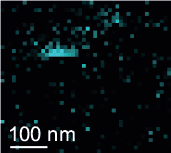
\includegraphics[width=0.3\textwidth]{img/chapitre1/figure12/sequentialScan.png}}\hspace{1em}
        \subfigure[\label{fig-echantillon-deteriore-b}]{%
            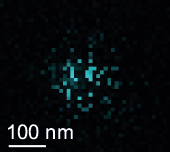
\includegraphics[width=0.3\textwidth]{img/chapitre1/figure12/randomScan.png}}
        \caption{\protect\subref{fig-echantillon-deteriore-a} Exemple d'échantillon détérioré par un faisceau trop énergétique. L'acquisition est réalisée ligne par ligne en commençant au pixel supérieur gauche. \`A un certain stade de l'acquisition, une structure apparaît puis disparaît soudainement. En effet, la structure a été détruite suite à une trop grande accumulation d'énergie, l'acquisition conventionnelle illuminant les positions successives. \protect\subref{fig-echantillon-deteriore-b} Acquisition d'une structure semblable avec un parcours aléatoire et la même énergie par pixel. La structure est elle-aussi détériorée, mais l'échantillonnage aléatoire permet de visualiser la particule avant sa disparition.
            \protect\label{fig-echantillon-deteriore}}
    \end{figure}

    \paragraph{Acquisition ligne par ligne v.s. aléatoire.} Une première solution pour réduire la détérioration de l'échantillon à énergie fixée consiste à échantillonner de manière aléatoire uniforme. En effet, l'acquisition ligne par ligne est très simple à implémenter, mais cette modalité détériore particulièrement l'échantillon puisqu'elle accumule des doses d'énergie sur des pixels voisins. Pour pallier ce problème, des travaux récents ont mis au point un obturateur coupant le faisceau au cours de l'acquisition standard~\cite{beche2016development}, permettant de limiter l'accumulation de charges au niveau local, au prix d'un sous-échantillonnage spatial. 
    %
    Afin d'échantillonner l'ensemble des pixels tout en protégeant l'échantillon, un module de balayage novateur basé sur FPGA a été mis au point au LPS~\cite{tararan2016random, zobelli2019spatial, tence2019following} dont le fonctionnement est décrit sur la figure~\ref{fig-random-scan}. Une de ses caractéristiques principales est de rendre le chemin d'acquisition hautement paramétrable où l'ensemble des positions spatiales sont stockées dans une table. L'ordre des pixels est mélangé aléatoirement lors d'une phase initiale, puis ce chemin aléatoire est chargé. 
    %
    Pour chaque nouvelle position à visiter, le module pilote des bobines magnétiques afin de positionner le faisceau sur l'échantillon tandis que l'acquisition du signal est désactivée à l'aide d'un obturateur de faisceau électrostatique. Une fois la position désirée atteinte, le faisceau illumine l’échantillon uniquement pendant le temps requis pour l’acquisition du signal, temps durant lequel la caméra est en mode d’exposition. Enfin, le faisceau est coupé et déplacé vers la position suivante.
    \begin{figure*}
        \centering
        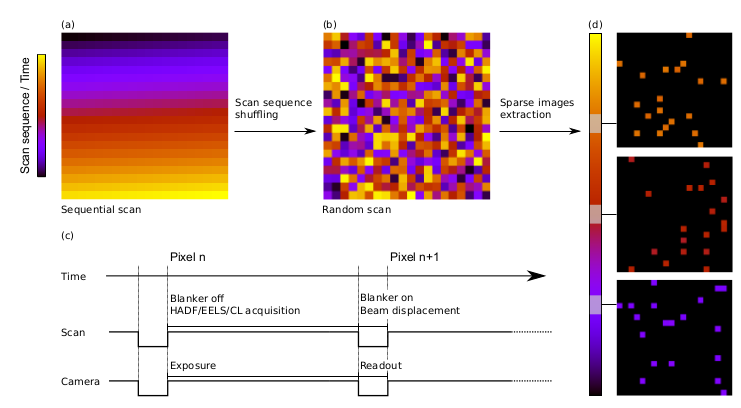
\includegraphics[width=\textwidth]{img/chapitre1/figure18/random-scan-2}
        \caption{\protect\label{fig-random-scan}Principe de l'acquisition ligne par ligne standard (a) et la séquence d'échantillonnage aléatoire (b). L'échelle de couleur représente l'ordre d'acquisition des pixels. (c) Représentation schématique de la synchronisation entre illumination, déplacement du faisceau, obstruction du faisceau, exposition et mesure. (d) Extraction d'images aléatoires partielles à certaines trames temporelles. La figure est issue de~\cite{zobelli2019spatial}.}
    \end{figure*}
    Cette technique d'acquisition permet de répartir la dose d'électron sur l'ensemble de l'échantillon. Cela est mis en évidence à la \cref{fig-echantillon-deteriore-b} puisque la structure spatiale est totalement visible pour une acquisition aléatoire tandis que l'échantillonnage ligne par ligne  détruit prématurément la structure, comme le montre la \cref{fig-echantillon-deteriore-a}. Cette technique permet donc d'augmenter l'énergie délivrée à l'échantillon pour une détérioration égale, et donc d'améliorer la qualité de l'image.
    
    
    \paragraph{Correction de la dérive de l'échantillon.} Comme expliqué à la \cref{sec-prop-eels}, l'échantillon n'est pas nécessairement stable au cours de l'acquisition puisque des gradients de température et des mouvements d'air le font dériver. Dans le cas d'une acquisition ligne par ligne, cela se manifeste par une déformation du réseau atomique, comme le montre la \cref{fig-drift}. Dans le cas d'un échantillonnage aléatoire, cela détériore grandement la résolution spatiale, particulièrement pour les échantillons à échelle atomique. 
    %
    En pratique, la dérive est limitée en laissant l'échantillon se stabiliser après insertion dans le microscope et en s'assurant que l'acquisition soit suffisamment rapide.
    %
    Pour corriger cela, une méthode consiste à extraire $K<P$ sous-acquisitions partielles de l'acquisition aléatoire complète. Chacune de ces acquisitions partielles est alors complétée indépendamment à l'aide d'une méthode de reconstruction (cf \cref{ch-chapter_2}) et le mouvement de l'échantillon est estimé. Les échantillons associés à chaque sous-acquisition sont alors recalés pour compenser la dérive. Cette méthode est appelée \emph{multi-trame} et a été implémentée avec succès en imagerie \gls{haadf} et \gls{eels}~\cite{zobelli2019spatial}. Cette méthode améliore sensiblement la qualité de l'image, mais reste encore très peu utilisée car lourde d'un point de vue expérimental. Enfin, dans le cas d'un échantillonnage ligne par ligne où l'échantillon dérive uniformément, il est également possible de corriger le défaut par déformation géométrique du réseau.

    \paragraph{Débruitage en post-traitement.} L'approche la plus simple pour limiter la détérioration de l'échantillon consiste à réduire la dose d'électrons et à débruiter les données en post-traitement. 
    %
    Pour cela, la technique la plus couramment utilisée pour de nombreuses données spectroscopiques revient à appliquer l'\gls{acp} aux données pour ne conserver que les composantes les plus puissantes, comme cela a été fait pour réduire le bruit spectral en imagerie à échelle atomique~\cite{bosman2007two,dudeck2012quantitative}, par exemple. Cette technique rapide et simple ne permet toutefois pas d'améliorer la qualité spatiale de l'image. D'autre part, certaines études ont mis en évidence des artefacts introduits par l'\gls{acp}, comme un biais présent dans le spectre reconstruit~\cite{lichtert2013statistical, spiegelberg2017can} ou encore l'ajout de structures initialement absentes \cite{mevenkamp2017mm}.
    %
    C'est pourquoi des techniques de débruitage par patch plus récentes et plus efficaces (\cf{} \cref{sec-art-patch}) ont été appliquées afin d'accroître le \gls{snr} du spectre-image tout en limitant les distorsions. Contrairement à l'ACP, celles-ci permettent de débruiter tant spatialement que spectralement. En particulier, des techniques non-locales comme Non-Local Means~\cite{mevenkamp2017mm, mevenkamp2020multimodal} et des approches par \gls{ad} avec apprentissage~\cite{trampert2018ultramicroscopy} ont été appliquées respectivement à des données \gls{eels} et  \gls{sem}. De même, un algorithme non-local appelé Local Low Rank (LLR)~\cite{spiegelberg2018local} a été proposé et appliqué avec succès à des images 2D \gls{haadf} et à des données 3D réalisées après concaténation de cartes d'abondance obtenues par imagerie \gls{stem}-\gls{eels}.
    %
    Cependant, cette façon de préserver l'échantillon pourrait ne pas suffire si la dose maximale autorisée est trop faible. En effet, l'image serait trop dégradée pour être efficacement débruitée et les structures fines pourraient ne plus être détectées. 
    
    
    \section{Positionnement de la thèse}\label{sec-positionnement-these}

    L'équipe STEM du \gls{lps} a très tôt étudié l'ensemble des stratégies présentée dans la section précédente en vue de prévenir la destruction d'échantillons sensibles. Plus précisément, cela a été motivé par l'implémentation du module de balayage décris précédemment afin de contrôler le chemin d'acquisition. Ce système est actuellement installé sur deux microscopes \gls{stem} :
    \begin{itemize}
        \item un VG-HB501 avec un pouvoir séparateur de l’ordre du nm (\cf{} \cref{fig-LPS-micro-a}),
        \item un Nion UltraSTEM 200 équipé d’un correcteur d’aberrations sphériques qui permet d’atteindre un pouvoir séparateur de l’ordre de 0,1 nm (\cf{} \cref{fig-LPS-micro-b}).
    \end{itemize}
    %
    \begin{figure*}
        \centering  % 0.8, 0.5
        \subfigure[\label{fig-LPS-micro-a}]{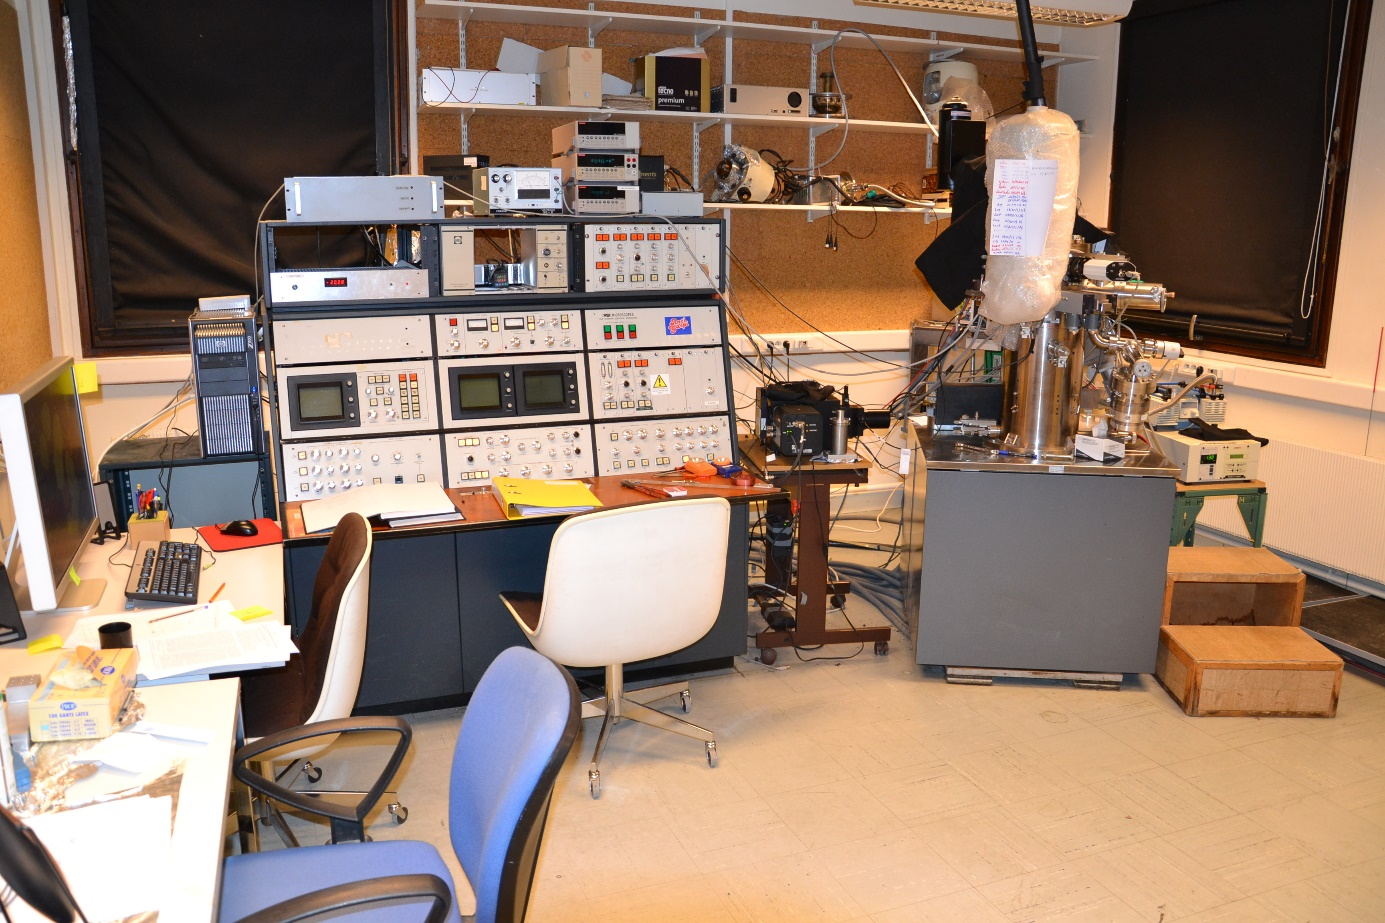
\includegraphics[width=0.5\textwidth]{img/chapitre1/figure13/VG.jpg}}
        \hspace{1em}
        \subfigure[\label{fig-LPS-micro-b}]{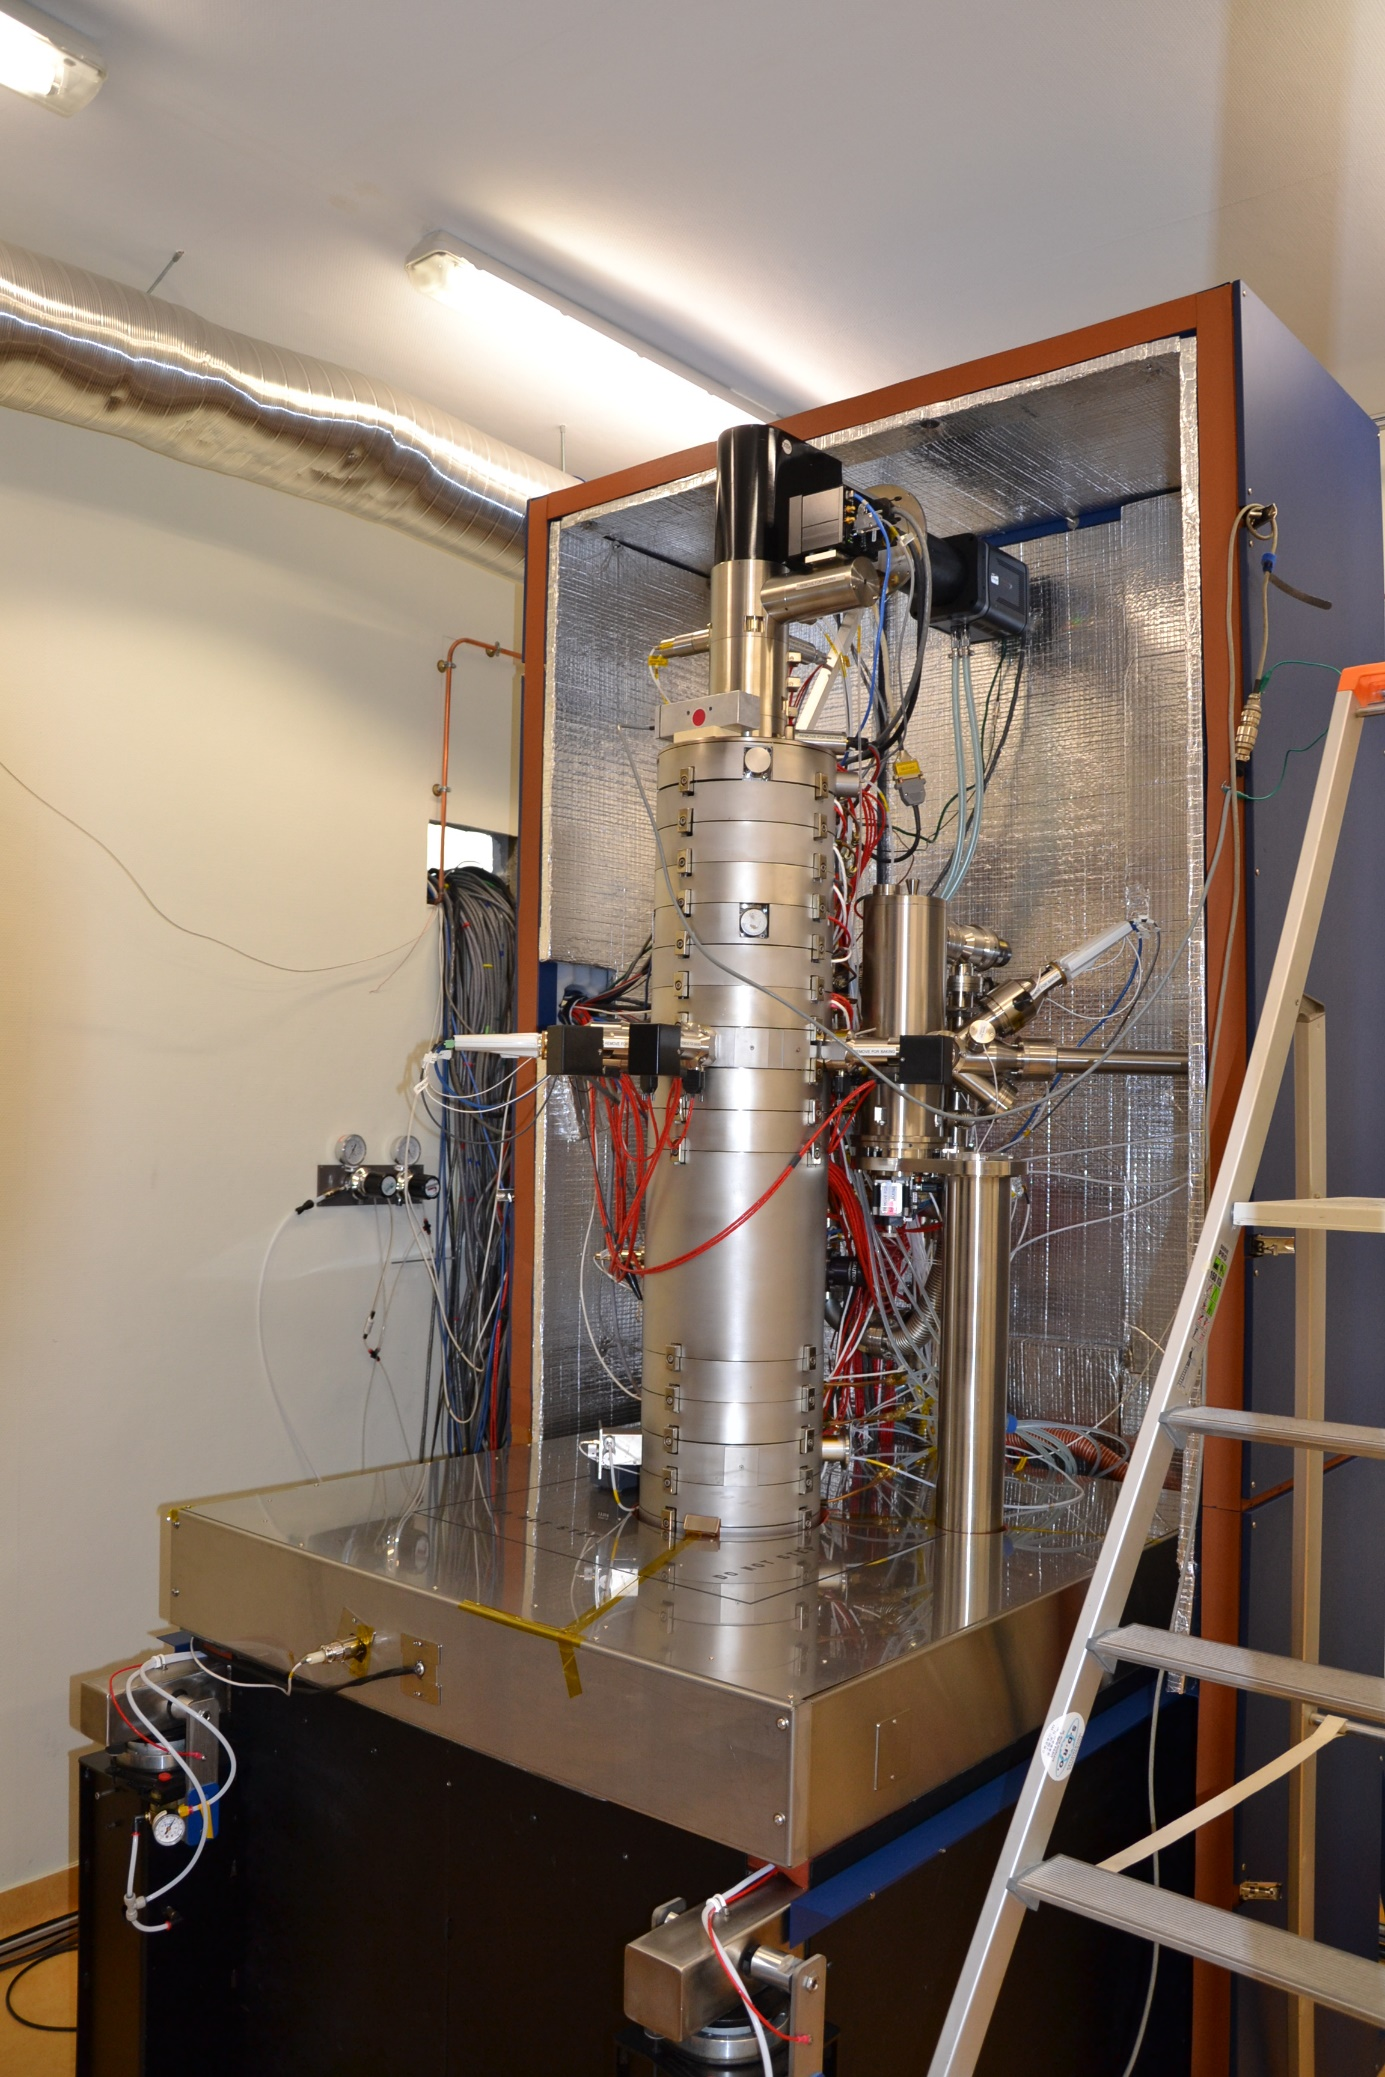
\includegraphics[width=0.4\textwidth]{img/chapitre1/figure13/NION.jpg}}
        \caption{Microscopes en service au \gls{lps} sur lesquels le mode d'acquisition aléatoire est implémenté. \subref{fig-LPS-micro-a} VG-HB501. \subref{fig-LPS-micro-b} Nion UltraSTEM 200.
            \protect\label{fig-LPS-micro}}
    \end{figure*}
    En couplant cette technique d'acquisition à des méthodes de débruitage performantes, on observe une grande amélioration de la qualité de l'acquisition, en particulier pour des temps d'exposition faibles ou des échantillons sensibles. 
    
    Cependant, la grande flexibilité du paramétrage du chemin d'acquisition ouvre la voie à une nouvelle alternative, celle d'accroître la dose d'électron par pixel (et donc le \gls{snr} associé), mais à ne visiter qu'un nombre réduit de positions spatiales en stoppant l'acquisition aléatoire avant son terme. Un algorithme de reconstruction d'image vient enfin compléter les positions manquantes en post-traitement. En paramétrant correctement la dose d'électrons par pixels et le nombre de positions visités, la dose d'électron utilisée est la même que pour les techniques d'acquisition standards et la dégradation de l'échantillon reste identique. 
    %
    Cette façon de procéder a motivé l'usage de techniques de reconstruction performantes issues de la communauté du traitement du signal et il s'agit d'un domaine de recherche très actif en microscopie \gls{stem}~\cite{beche2016compressed,stevens2014potential} et \gls{sem}~\cite{anderson2013sparse} entre autres.
    %
    D'autre part, les performances de cette approche sont intimement liées au choix du chemin d'acquisition et différents travaux présentés à la \cref{sec-art-micro} se sont intéressés à la part d'aléatoire et de régularité à introduire dans ce choix. Certains d'entre eux ont également proposé d'acquérir l'image partielle de manière dynamique en déterminant à chaque instant d'acquisition le pixel à visiter à l'instant suivant.
    %
    Les deux protocoles d'acquisition (débruitage et reconstruction) ont à la fois des avantages et des inconvénients. D'une manière générale, une acquisition à faible dose fournit des informations spatiales plus riches tandis que les données partiellement acquises ont un contenu spectral plus riche. Déterminer quelle approche est la meilleure n'est pas trivial et des études récentes ont comparées ces deux approches~\cite{trampert2018ultramicroscopy} en se basant sur des expériences réalisées sur des images synthétiques et réelles.
    
    Enfin, les techniques de reconstruction sont encore assez marginales dans l'équipe et n'ont été utilisées qu'en cathodoluminescence~\cite{zobelli2019spatial}. 
    %
    Les efforts récents se sont concentrés sur la reconstruction en ligne du spectre-image dans une bande et sa visualisation afin de déterminer si l'élément d'intérêt est présent dans la région observée%
    %
    \footnote[][-2\baselineskip]{%
    Il ne s'agit pas ici de reconstruire le spectre-image complet, mais seulement de sommer des bandes du spectre-image incomplet autours d'un seuil d'intérêt, puis de reconstruire l'image 2D partielle obtenue. Il ne s'agit pas d'une technique d'analyse complètement fiable puisque l'on visualise aussi les effets des seuils précédents, mais cela permet de donner une première idée quant à la présence de l'élément cherché au cours de l'acquisition.}%
    . 
    Cela permettrait d'arrêter prématurément l'acquisition si l'élément est absent, préservant ainsi l'échantillon et accélérant la recherche d'une zone d'intérêt. 
    %
    Une fois ceci fait, des techniques de reconstruction hors-ligne efficaces (et possiblement gourmandes en ressources) seraient nécessaires afin de reconstruire les spectre-images avec une grande précision. Enfin, l'échantillonnage partiel pourrait être utilisé sur les zones étudiées afin de préserver l'échantillon tout en maximisant le \gls{snr}, l'image complète étant restituée a posteriori.
    
    Le travail de thèse présenté dans ce manuscrit a pour but d'évaluer l'apport de l'échantillonnage partiel dans l'acquisition d'échantillons sensibles en imagerie STEM-EELS. Plus précisément, je m'intéresse tout particulièrement à proposer des techniques de reconstruction rapides et efficaces à mettre en \oe{}uvre au cours de l'acquisition. Celles-ci seront comparées à des méthodes de reconstruction plus longues constituant l'état de l'art. Dans ce but, le chapitre~\ref{ch-chapter_2} fera le point sur les méthodes de reconstruction d'images et sur leur utilisation dans la communauté en microscopie.
    
    
    
    
    
    



% ---

\chapter{Etat de l'art}
\dochaptoc
\label{ch-chapter_2}

%
\section{La reconstruction : un problème d'inpainting}

\subsection{Contexte}


De nombreux problèmes en traitement de l'image consistent à corriger une région détériorée ou manquante et, suivant les situations, le masque spécifiant les zones manquantes est plus ou moins structuré. En retouche photographique, par exemple, le masque indiquant les régions à enlever d'une prise de vue~\cite{criminisi2004region} est fortement structuré et les structures sont fines (comme la grille visible à la figure~\ref{fig-inpainting-b}) ou grosses (personnages). Au contraire, le masque peut être très faiblement structuré et réparti, comme à la figure~\ref{fig-inpainting-e} où l'image est aléatoirement et partiellement acquise. Outre les situations où l'acquisition est volontairement lacunaire, les données peuvent souffrir de dysfonctionnements du capteur~\cite{zhang2013hyperspectral} et des bandes (resp. des pixels) peuvent être détériorés, conduisant à un masque fortement structuré et fin (resp. faiblement structuré et réparti).

Pour corriger ces défauts, de nombreuses méthodes proposées ces dernières décennies complètent les régions masquées en se basant sur l'information disponible et non-corrompue. Ainsi, les travaux de Bertalmio \etal{}~\cite{bertalmio2000image} se sont inspirés des techniques de restaurateurs en peinture employés par les musées et ont introduit le terme d'\emph{inpainting} pour désigner ces méthodes de complétion. Des exemples d'inpainting sont affichés aux \crefrange{fig-inpainting-a}{fig-inpainting-c} (resp. \crefrange{fig-inpainting-d}{fig-inpainting-f}) pour un masque structuré fin (resp. pour un masque réparti aléatoire). 

\begin{figure}[b]
    \centering
    \subfigure[\label{fig-inpainting-a}]{
        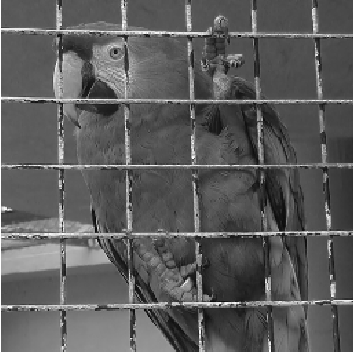
\includegraphics[width=0.25\textwidth]{img/chapitre2/figure1/initial-2.png}}\hspace{1em}
    \subfigure[\label{fig-inpainting-b}]{
        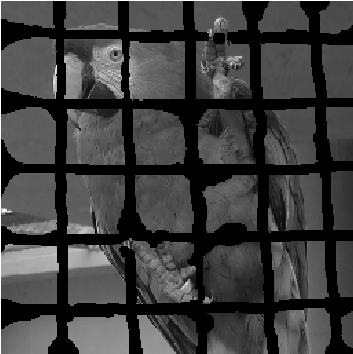
\includegraphics[width=0.25\textwidth]{img/chapitre2/figure1/mask-2.png}}\hspace{1em}
    \subfigure[\label{fig-inpainting-c}]{
        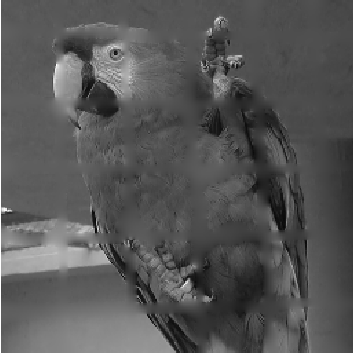
\includegraphics[width=0.25\textwidth]{img/chapitre2/figure1/final-2.png}}\\
    %
    \subfigure[\label{fig-inpainting-d}]{
        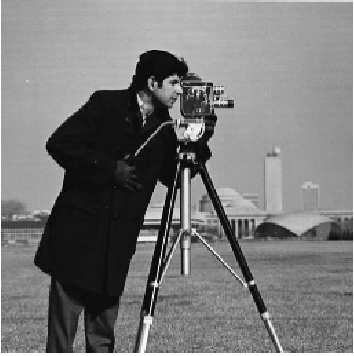
\includegraphics[width=0.25\textwidth]{img/chapitre2/figure2/initial.png}}\hspace{1em}
    \subfigure[\label{fig-inpainting-e}]{
        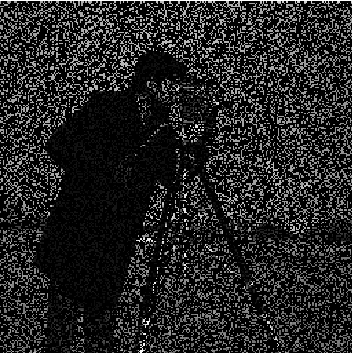
\includegraphics[width=0.25\textwidth]{img/chapitre2/figure2/mask.png}}\hspace{1em}
    \subfigure[\label{fig-inpainting-f}]{
        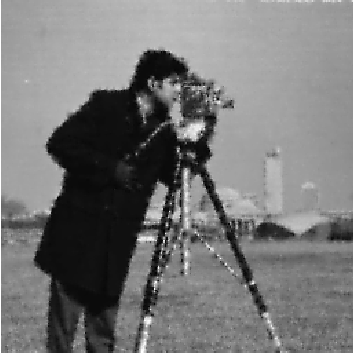
\includegraphics[width=0.25\textwidth]{img/chapitre2/figure2/final.png}}
    \caption{Exemple d'inpainting extrait de~\protect\cite{peyre2011numerical}. \protect\subref{fig-inpainting-a} Exemple d'image destinée à la retouche photographique. \protect\subref{fig-inpainting-b} Les pixels composant la grille sont masqués. \protect\subref{fig-inpainting-c} Résultat après inpainting. \protect\subref{fig-inpainting-d} Exemple d'acquisition complète. \protect\subref{fig-inpainting-e} La même image acquise partiellement. \protect\subref{fig-inpainting-f} Résultat après inpainting.
        \protect\label{fig-inpainting}} 
\end{figure}


La complétion peut être considérée comme un problème inverse dont le modèle d'acquisition est donné à la section suivante~\ref{subsec-direct-inverse-problem}. Plus largement, elle s'inscrit dans le cadre général de l'acquisition comprimée qui fournit des méthodes de restauration avec des garanties théoriques pour les problèmes inverses linéaires sous-déterminés. Les travaux d'Emmanuel Candès, Justin Romberg, Terence Tao et David Donoho~\cite{candes2006near, candes2006stable, donoho2006compressed} ont révolutionné le domaine du traitement du signal. Ceux-ci ont par exemple démontré qu'une image acquise avec une fréquence d'échantillonnage inférieure à celle de Nyquist pouvait être restaurée de manière exacte sous certaines conditions (dont une spécifiant que les données doivent être parcimonieuses dans une certaine base). Cette technique a été appliquée avec succès dans de nombreux domaines incluant l'\gls{irm}~\cite{boyer_algorithm_2014}, l'imagerie ultrasonique~\cite{quinsac_bayesian_2011}, l'astronomie~\cite{bobin_compressed_2008} ou la tomographie en microscopie~\cite{binev2012compressed, jacob2019MM, jacob2018MM}. %
%
Ces résultats ont rendu populaire les problèmes d'inpainting et il s'agit d'un domaine de recherche très actif en microscopie \gls{stem}~\cite{beche2016compressed,stevens2014potential} et \gls{sem}~\cite{anderson2013sparse} entre autres.


La technique d'inpainting est généralement associée à la reconstruction d'images 2D, mais elle s'étend au-delà pour les images multi-dimensionnelles dont une partie des voxels (l'équivalent des pixels pour une image multi-dimensionnelle) sont manquants.
%
La stratégie d'acquisition partielle décrite à la \cref{sec-ech-sensibles} s'inscrit dans ce contexte. En effet, la sonde ne visite qu'une partie de l'échantillon en suivant un chemin généralement aléatoire. Il en résulte des données spatialement sous-échantillonnées que les techniques d'inpainting peuvent compléter.
%
Notons également que ce schéma d'acquisition spatial ne s'accompagne pas d'un sous-échantillonnage spectral puisque, pour chaque position spatiale, le spectromètre \gls{eels} sépare simultanément toutes les pertes d'énergie conduisant à une acquisition complète du spectre. Il en résulte que le masque pour une telle stratégie est \emph{fortement structuré}.


\subsection{Modélisation du problème d'inpainting}\label{subsec-direct-inverse-problem}

Notons $\gls{Y}\in\mathbb{R}^{\gls{M}\times\gls{P}}$ la matrice qui correspondrait aux données \gls{eels} complètes composées de \gls{P} pixels et de \gls{M} canaux. 
%
Comme expliqué à la \cref{sec-ech-sensibles}, faire l'acquisition complète du spectre-image \gls{Y} n'est pas toujours possible dû à la détérioration introduite par le faisceau d'électron sur l'échantillon et c'est pourquoi un sous-échantillonnage spatial est envisagé, comme expliqué à la section~\ref{sec-positionnement-these}.
%
Ainsi, les spectres complets sont acquis en \gls{N} positions parmi \gls{P}, il en résulte un taux d'échantillonnage $\gls{r}=\gls{N}/\gls{P}$. L'ensemble des indices des \gls{N} positions spatiales visitées ainsi que la matrice d'observation sont respectivement notés \gls{I} et \gls{Yi}, où \gls{Yi} est la matrice de taille \taille{M}{N} rassemblant les $N$ colonnes de \gls{Y} indexées par \gls{I}. %

Nous avons vu à la \cref{sec-prop-eels} que le bruit présent dans les données est le mélange de plusieurs contributions avec chacune leur propriétés statistiques. Il en résulte que quantifier chacune de ces contribution est complexe en pratique et les modèles classiquement retenus dans la littérature sont les bruits poissonnien~\cite{egerton2011electron, mevenkamp2015poisson, stevens2018apl}, gaussien~\cite{stevens2014potential, binev2012compressed} et mixte poisson-gaussien~\cite{sanders2020inpainting}. Dans ce manuscrit, nous choisirons de modéliser la détérioration des données avec un bruit indépendant, additif et gaussien. Deux raisons motivent ce choix. D'abord, les paramètres du bruit sont difficiles à caractériser en pratique, si bien que le bruit gaussien plus simple est préféré. Ensuite, les expériences conduites à l'annexe~\ref{sec-bruit-mixte} avec un modèle de bruit mixte n'ont pas permis de mettre en évidence une perte de performances significative par rapport à un modèle gaussien seul. De plus, si une composante poissonnienne émerge particulièrement, des techniques de stabilisation de variance comme la transformée de Anscombe~\cite{anscombe1948transformation} permettent de \guillemets{convertir} le bruit mixte en un bruit gaussien.

Finalement, la matrice observée \gls{Yi} peut être décrite par le modèle suivant :
\begin{equation}
    \gls{Yi} = \gls{X}_{\gls{I}} + \gls{E}
\end{equation}
où \gls{X} est l'image idéle et \gls{E} est un terme résiduel représentant l'erreur de modèle et le bruit d'acquisition. Les éléments de \gls{E} sont supposés être indépendants et identiquement distribués selon une loi gaussienne centrée d'écart type \gls{sig}.

Le problème de reconstruction consiste à estimer un spectre-image de taille \taille{M}{P} complet (et possiblement débruité) \gls{X} à partir de \gls{Yi}. Cependant, cette tâche est mal posée puisque le nombre de paramètres \gls{P}\gls{M} est supérieur au nombre d'observations \gls{N}\gls{M} et la suite de ce chapitre étudiera les approches possibles pour résoudre ce problème inverse.


%
\section{Les différentes classes d'inpainting}

Cette section présente les méthodes de reconstructions classiquement rencontrées dans la littérature en les classant en cinq sections : les techniques d'interpolation, les techniques de \gls{mc} régularisés, les techniques par diffusion, les techniques par patch et les techniques par réseaux de neurones.


\subsection{Les techniques d'interpolation}\label{sec-interpolation}

\paragraph{Présentation du problème d'interpolation.} Le problème d'inpainting peut être vu comme un problème d'interpolation. L'image est alors définie par une fonction $f:\mathbb{R}^3\rightarrow \mathbb{R}$ associant chaque voxel $p\in\mathbb{R}^3$ à une valeur $f(p)\in\mathbb{R}$, connue en un ensemble de points $(s_k)_{k\in\gls{I}}$. Reconstruire l'image, c'est estimer les valeurs prises par $f$ sur un ensemble de points $(m_k)_{k\in \gls{I}^c }$ définis par le masque qu'il soit structuré ou non. 
%
Ce problème est facile en 1D et reste simple en dimension trois à condition que les points masqués soient répartis suivant une maille générée par trois ensembles de coordonnées $\mathcal{J}_x$, $\mathcal{J}_y$, $\mathcal{J}_{eV}$. L'interpolation est plus difficile dans le cas général, comme dans notre situation où le masque est aléatoirement et uniformément généré. L'espace doit alors être découpé en éléments de base, puis la fonction est interpolée sur ces éléments. Par exemple, en 2D, l'enveloppe convexe du nuage de points échantillonnés peut être découpée en un ensemble de triangles à l'aide de la triangulation de Delaunay présentée à l'annexe~\ref{abstr-voronoi-delaunay}. En particulier, chaque triangle de la triangulation a pour sommets des points du nuage et aucun point échantillonné ne se situe à l'intérieur du cercle circonscrit au triangle. L'avantage principale de cette triangulation sa faible complexité : $\mathcal{O}(|\gls{I}|\log |\gls{I}|)$~\cite{lee1980two}, voire $\mathcal{O}(|\gls{I}|\log \log |\gls{I}|)$~\cite{dwyer1987faster} dans de nombreux cas.

\paragraph{Interpolation par \Glsentrylong{ppv}.} L'interpolation par \gls{ppv} est la technique d'interpolation la plus simple et la moins coûteuse. Elle consiste à associer à chaque point à interpoler la valeur prise par $f$ au point échantillonné $s_{k}$ le plus proche. Cela consiste à associer $f(s_{k})$ à tout point $x$ appartenant à la cellule de Voronoi de $s_{k}$, définie par l'ensemble des points plus proches de $s_k$ que de tout autre point de $(s_{k'})_{k'\neq k}$. Le diagramme de Voronoi constitué de l'ensemble des cellules est décrit à l'annexe~\ref{abstr-voronoi-delaunay} et a la même complexité que la triangulation de Delaunay. Cette méthode, bien que très peu coûteuse, est aussi la moins efficace puisque la fonction interpolée est constante par morceaux, ce qui entraîne une erreur de reconstruction élevée. Cela est particulièrement visible sur l'exemple d'interpolation \gls{ppv} donné aux figures \ref{fig-interpolation-a} et \ref{fig-interpolation-d} puisque les cellules de Voronoi apparaissent clairement sur l'image.

Pour lisser davantage la fonction interpolée, une solution consiste à associer au point à interpoler $x$ une pondération des valeurs prises par les points $(s_k)_k$ voisins, c'est-à-dire
\begin{equation}\label{eq-weighted-interp}
    \hat{f}(x) = \sum_{k\in\gls{I}} w_k(x) f(s_k)
\end{equation}%
\begin{marginfigure}%
    \centering
    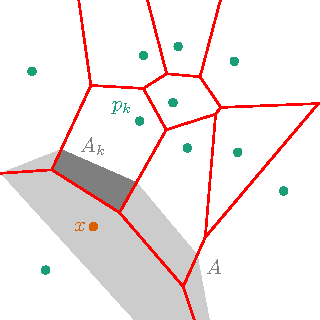
\includegraphics[]{img/chapitre2/figure3/Voronoi_Natural.pdf}
    \caption{Illustration de la méthode par plus proches voisins naturels. Le diagramme de Voronoi associé à l'ensemble de points $(s_k)_k$ connu (en vert) est affiché (en rouge). Lorsque le nouveau point (en orange) est ajouté, une cellule (en gris) est ajoutée au diagramme.}
    \label{fig-natural-weight}
\end{marginfigure}%
\noindent où $w_k(x)$ est le poids de $x$ associé au point échantillonné $s_k$ (la somme des poids vaut 1). Une approche classique consiste à évaluer le diagramme de Voronoi de $(s_k)_{k\in\gls{I}}$ (en rouge à la \cref{fig-natural-weight}), puis une deuxième fois en ajoutant $x$ (la cellule supplémentaire est en gris à la \cref{fig-natural-weight}). Si l'on note $A_k$ l'aire de l'intersection entre cette nouvelle cellule et la cellule précédemment associée à $s_k$ et $A$ l'aire de la nouvelle cellule associée à $x$, alors on pose $w_k(x)=A_k/A$. Cette approche, appelée interpolation par plus proches voisins naturels~\cite{sibson1981interpreting,cazals2006delaunay}, donne de meilleurs résultats que l'interpolation par plus proche voisins, mais elle est aussi plus lourde d'un point de vue calculatoire.

\paragraph{Interpolation pour des ordres supérieurs.} Comme expliqué plus haut, l'interpolation dans le cas multidimensionnel est généralement réalisée en ajustant une fonction d'ordre fixe sur chaque simplexe issu de la triangulation de Delaunay. Ainsi, l'interpolation \gls{ppv} ajuste une fonction constante par morceau sur les sommets du simplexe. Des ordres supérieurs peuvent être utilisés, comme l'interpolation linéaire ou cubique en 1D correspondant respectivement à des fonctions d'ordre 1 et 3. En 2D, cela consiste à ajuster des plans ou des surfaces cubiques par régression aux sommets du triangle. En plus grande dimension, l'interpolation linéaire est réalisée par interpolation barycentrique~\cite{hormann2014barycentric}. Les figures~\ref{fig-interpolation-b}, \ref{fig-interpolation-c}, \ref{fig-interpolation-e} et \ref{fig-interpolation-f} permettent de visualiser le résultat de la régression dans les cas linéaire et cubique.
  
\begin{figure}[h]
    \centering
    \subfigure[\label{fig-interpolation-a}\gls{ppv}]{
        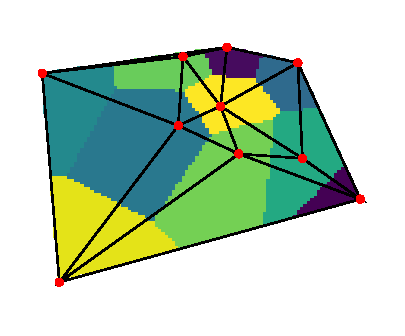
\includegraphics[width=0.29\textwidth]{img/chapitre2/figure4/nearest.pdf}}\hspace{1em}
    \subfigure[\label{fig-interpolation-b}Interpolation linéaire]{
        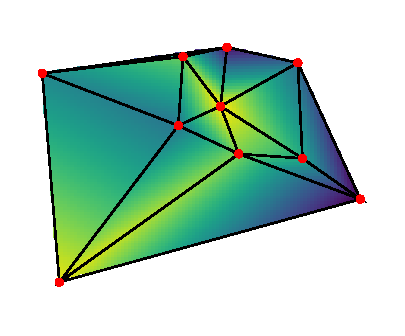
\includegraphics[width=0.29\textwidth]{img/chapitre2/figure4/linear.pdf}}\hspace{1em}
    \subfigure[\label{fig-interpolation-c}Interpolation cubique]{
        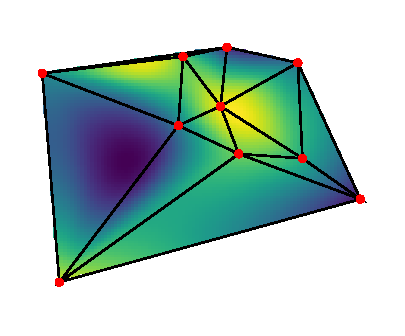
\includegraphics[width=0.29\textwidth]{img/chapitre2/figure4/cubic.pdf}}\\
    \subfigure[\label{fig-interpolation-d}\gls{ppv}]{
        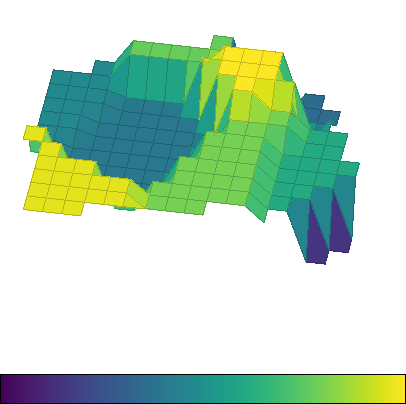
\includegraphics[width=0.29\textwidth]{img/chapitre2/figure4/surf_nearest.pdf}}\hspace{1em}
    \subfigure[\label{fig-interpolation-e}Interpolation linéaire]{
        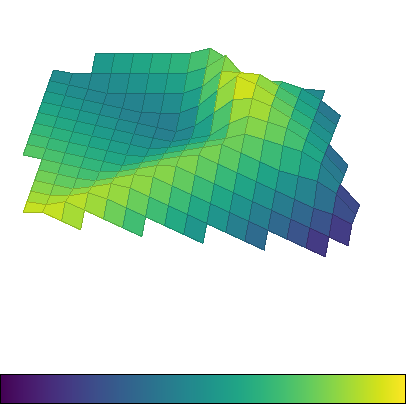
\includegraphics[width=0.29\textwidth]{img/chapitre2/figure4/surf_linear.pdf}}\hspace{1em}
    \subfigure[\label{fig-interpolation-f}Interpolation cubique]{
        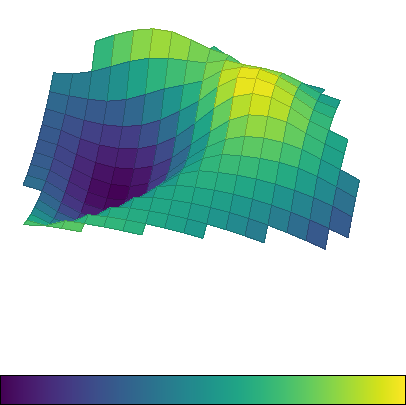
\includegraphics[width=0.29\textwidth]{img/chapitre2/figure4/surf_cubic.pdf}}
    \caption{Exemple d'interpolation sur un nuage de points aléatoirement généré (en rouge). La fonction est interpolée sur l'enveloppe convexe en s'appuyant sur la triangulation de Delaunay représentée en noir. \protect\subref{fig-interpolation-a} Interpolation \gls{ppv}. \protect\subref{fig-interpolation-b} Interpolation linéaire. \protect\subref{fig-interpolation-c} Interpolation cubique. Les fonctions interpolées sont également représentées dans le même ordre sous forme de surfaces aux figures~\subref{fig-interpolation-d} à \subref{fig-interpolation-f} (la résolution spatiale est diminuée pour des raisons d'affichage).
        \protect\label{fig-interpolation}}
\end{figure}


\paragraph{Avantages et inconvénients.} Les méthodes d'interpolation ont pour principal avantage leur faible complexité et leur rapidité, ce qui en font des méthodes populaires en reconstruction en ligne~\cite{sibson1981interpreting, cazals2006delaunay, trampert2018ultramicroscopy}. Néanmoins, elles ne sont pas robustes puisqu'elles s'ajustent aux valeurs disponibles elles-mêmes corrompues. Elles ne permettent pas d'introduire plus d'information a priori que l'ordre de la fonction à interpoler.

\subsection{Les techniques par \glsentrylong{mc} régularisés}\label{sec-MC-regul}

Une approche \emph{variationelle} en inpainting est une méthode calculant l'image reconstruite en minimisant une fonction objectif. En particulier, une technique par \gls{mc} régularisés fournit une image reconstruite \gls{Xh} en résolvant le problème de minimisation suivant~\cite[Section~6.3]{boyd2004convex}
\begin{equation}\label{eq-MC-regul}
    \gls{Xh} = \argmin_{\gls{X}} \frobnorm{\gls{X}_{\gls{I}} - \gls{Yi}} + \lambda \mathcal{R}(\gls{X})
\end{equation}
où $\frobnorm{\gls{X}_{\gls{I}} - \gls{Yi}}$ est le terme d'attache aux données et où l'opérateur $\mathcal{R}$ est une régularisation. Le scalaire $\lambda$ permet d'ajuster l'importance de la régularisation par rapport au terme d'attache aux données. Cette formulation peut s'interpréter comme (si on choisi le paradigme bayésien) l'estimateur du \gls{map} puisque la formule de Bayes donne la fonction de vraisemblance $P(\gls{X}|\gls{Yi}) \propto P(\gls{Yi}|\gls{X}) P(\gls{X})$. En considérant l'opposé de la log-vraissemblance, l'estimée est l'image \gls{X} minimisant la fonction
\begin{equation}
    -\log P(\gls{X}|\gls{Yi}) \propto
    \underbrace{-\log P(\gls{Yi}|\gls{X})}_{\frobnorm{\gls{X}_{\gls{I}} - \gls{Yi}}}
    \underbrace{- \log P(\gls{X})}_{\mathcal{R}(\gls{X})}.
\end{equation}
Il en résulte que le terme d'attache aux données est choisi en fonction du modèle statistique du bruit tandis que la régularisation dépend de l'information a priori disponible pour \gls{X}. Ces méthodes gèrent donc mieux la connaissance du bruit que les techniques d'interpolation et sont ainsi plus robustes. En particulier, le terme d'attache aux données pour un bruit additif gaussien blanc est la fonction coût \gls{mc} $\frobnorm{\gls{X}_{\gls{I}} - \gls{Yi}}$. D'autres fonctions peuvent être utilisés lorsque la statistique du bruit est différente, comme la norme $\ell_1$ pour un bruit laplacien~\cite{frecon2017bayesian} ou la divergence de Kullback–Leibler pour un bruit poissonnien~\cite{ono2013poisson}. Notons encore que les problèmes de \gls{mc} régularisés conviennent que le masque soit structuré ou non et qu'ils sont également utilisés pour la complétion en se basant sur une triangulation, comme c'est le cas en ajustement de surface~\cite{zhong2016surface,cazals2006delaunay}.

Un choix particulièrement classique pour la régularisation est la fonction quadratique $\mathcal{R}(\gls{X}) = \frobnorm{\gls{X}}$, on parle alors de régularisation de Tikhonov. L'avantage de cette forme est que la solution est  donnée par une expression mathématique directe, ne nécessitant qu'une inversion de matrice. La loi a priori de \gls{X} est gaussienne centrée et promeut des données d'amplitude bien répartie autours de la moyenne.

Les techniques de \gls{mc} régularisés sont également d'un intérêt particulier dans le cas de données  parcimonieuses, c'est-à-dire dont la proportion d'entrées non nulles est faible. Dans ce cas, la régularisation idéale est la pseudo-norme $\ell_0$ \footnote{La pseudo-norme $\ell_0$ de \gls{X} vaut le nombre d'entrées non-nulle de \gls{X}. Il ne s'agit pas d'une norme puisque $||\alpha\gls{X}||_0 = ||\gls{X}||_0$ pour tout scalaire $\alpha$ non nul.} puisque celle-ci contraint le nombre d'éléments non-nuls. Malheureusement, résoudre ce problème d'estimation est très compliqué en pratique puisque la norme $\ell_0$ n'est pas convexe et on lui préfère généralement sa relaxation convexe : la norme $\ell_1$ définie par $||\gls{X}||_1 = \sum |\gls{X}_{ij}|$. Cette méthode est souvent appelée Lasso~\cite{tibshirani1996regression} de l'acronyme \emph{least absolute shrinkage and selection operator}. Enfin, il faut noter qu'utiliser la norme $\ell_1$ comme régularisation biaise le résultat. Pour corriger cela, des travaux ont proposé de résoudre le problème inverse en deux temps. D'abord, la technique Lasso est appliquée afin de déterminer les entrées non-nulles de l'estimée. Ensuite, une régression des moindres carrés est réalisée sur ce support. Cette méthode en deux temps est appelée post-LS (pour Least Square) ou encore \emph{refitting}~\cite{belloni2013least, lederer2013trust, deledalle2017clear}.

Utiliser une norme de $\gls{X}$ comme régularisation n'est pas toujours adaptée à l'information a priori disponible,  et l'on préfère généralement pénaliser $\mathcal{A}\gls{X}$ où $\mathcal{A}$ est un opérateur linéaire adapté. Ainsi, une alternative très populaire en traitement du signal consiste plutôt à contraindre le gradient de l'image $\nabla\gls{X}$, conduisant à une régularisation $\mathcal{R}(\gls{X})=\frobnorm{\nabla\gls{X}}$, on parle aussi d'énergie de Sobolev. Cela produit une image lissée. De même, la régularisation $\ell_1$ peut être couplée avec un opérateur linéaire $\mathcal{A}$ pour favoriser la parcimonie du signal dans un cas particulier, par exemple :
\begin{itemize}
    \item si $\mathcal{A}$ est un changement de base telle que $\mathcal{A}\gls{X}$ soit parcimonieuse, la régularisation $||\mathcal{A}\gls{X}||_1$ est adaptée,
    \item si $\mathcal{A}$ est l'opérateur de gradient spatial discret $\nabla$, la régularisation $||\nabla \gls{X}||_1$ appelée \gls{tv} promeut une image ayant peu de contours (l'image résultante est constante par morceaux).
\end{itemize}


\subsection{Les techniques par diffusion}

La diffusion est un processus physique intuitif tendant à équilibrer les différences de concentration au sein d'un fluide sans créer ou détruire de masse. Ce phénomène est régi par l'équation de diffusion suivante
\begin{equation}
    \frac{\partial u}{\partial t} \triangleq \dot{u}(x, y, t) = \mathrm{div} (D(x, y)\cdot \nabla u)
\end{equation}
où $u$ est la concentration, $D$ est le coefficient de diffusion et $\nabla$ est l'opérateur gradient. En traitement de l'image, on identifie la concentration avec la valeur en niveau de gris prise en une position particulière. Si le coefficient de diffusion est constant sur toute l'image, on parle de diffusion \emph{isotrope}, sinon, on parle de diffusion \emph{anisotrope}.

La technique de diffusion la plus simple est la diffusion isotrope en débruitage, conduisant au problème aux dérivées partielles suivant\footnote{Cette équation correspond aussi à l'équation de la chaleur dans le cas où il n'y a pas de source de chaleur.}
\begin{align}
&\dot{u} = D \cdot \Delta u\\
&u(\cdot, t=0) = y
\end{align}
où $\Delta$ est l'opérateur de laplacien spatial discret et $y$ est l'image bruitée. Ce problème est équivalent à un filtrage avec un noyau gaussien d'écart-type $\sqrt{2t}$\footnote{L'image resultante en diffusion n'est pas l'image $u(\cdot, t=\infty)$ puisque celle-ci est constante (la diffusion tend à égaliser les niveaux de gris). Il faut choisir un instant $t^*$ où arrêter la trajectoire et l'image resultante est $u(\cdot, t^*)$.} \cite{weickert1998anisotropic}. Le problème de cette technique est que la diffusion introduit un flou sur les contours de l'image. C'est pourquoi Perona et Malik~\cite{perona1990scale} ont proposé la diffusion anisotropique pour préserver les contours de l'image. Le coefficient de diffusion est diminué au niveau des contours tandis qu'il reste élevé au sein de zones homogènes. Le problème résultant s'écrit
\begin{align}
    &\dot{u}(x, y, t) = \mathrm{div} (D(|\nabla u|^2)\cdot \nabla u)\\
    & D(s) = \frac{1}{1+s^2/\lambda^2} \quad \text{pour $\lambda > 0$}
\end{align}

La technique de diffusion ne suffit cependant pas pour l'inpainting puisque la structure n'est pas propagée et un transport de matière doit être ajouté. Les travaux de Bertalmio \textit{et al.}~\cite{bertalmio2000image} ont été pionniers dans ce domaine et ont été à l'origine du terme \emph{inpainting}. S'inspirant des techniques de restauration en art, ils ont envisagé une technique par transport de matière propageant l'information le long de lignes de niveau (les lignes reliant les points de l'image ayant le même niveau de gris) dans le cas où le masque est structurée. Un terme de diffusion anisotrope était ajouté afin d'éviter que les lignes de niveau ne se croisent. D'autres techniques basées sur la variation totale on suivi~\cite{shen2002mathematical, chan2001nontexture} mais le principe fondamental consiste à propager la structure.

Ces techniques sont très bien adaptées aux images pour lesquelles le masque est très structurée, mais elles ne conviennent pas lorsque l'information est répartie. En effet, ces techniques reposent sur la propagation de contour. Dans le cas où les données sont réparties, aucun contour ne peut être propagé. C'est pourquoi nous n'utiliserons pas ces méthodes dans ce manuscrit.


\subsection{Les techniques par patch}\label{sec-art-patch}

Une extension des méthodes variationelles exploite la redondance spatiale dans l'image (la figure~\ref{fig-redondance-spatiale-search} illustre cette propriété), on parle alors de \emph{méthode par patch} ou \emph{examplar-based}. Elles constituent un ensemble de méthodes très populaires et performantes dont l'intérêt n'a cessé de grandir ces dernières décennies afin de résoudre des problèmes inverses comme le débruitage, l'inpainting ou la déconvolution.

\begin{figure}
    \centering
    \subfigure[\label{fig-redondance-spatiale-search}]{
        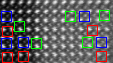
\includegraphics[width=0.7\textwidth]{img/chapitre2/figure5/search.png}}\\
    \subfigure[Atome rouge\label{fig-redondance-spatiale-dic1}]{
        \includegraphics[width=0.25\textwidth]{img/chapitre2/figure5/dico_red.png}}\hfill
    \subfigure[Atome vert\label{fig-redondance-spatiale-dic2}]{
        \includegraphics[width=0.25\textwidth]{img/chapitre2/figure5/dico_green.png}}\hfill
    \subfigure[Atome bleu\label{fig-redondance-spatiale-dic3}]{
        \includegraphics[width=0.25\textwidth]{img/chapitre2/figure5/dico_blue.png}}
    \caption{Illustration de la redondance spatiale en imagerie haute résolution. Une image \gls{haadf} est affichée à la figure~\subref{fig-redondance-spatiale-search} et trois familles de patch sont représentées en rouge, vert et bleu. Les patchs appartenant à une famille donnée sont tous semblables bien que éloignés dans l'image, confirmant l'hypothèse selon laquelle le contenu spatial de l'image est redondant. Les trois premiers atomes d'un dictionnaire appris à l'aide de la méthode mini-batch~\cite{mairal2009online} sont représentés aux figures~\subref{fig-redondance-spatiale-dic1} à \subref{fig-redondance-spatiale-dic3} et correspondent respectivement aux familles de patchs rouge, verte et bleue.
        \protect\label{fig-redondance-spatiale}}
\end{figure}

Ces méthodes sont à opposer aux techniques dites \emph{locales} où une valeur est corrigée en ne la comparant qu'avec son voisinage, comme lorsqu'une image est convoluée avec un masque gaussien en débruitage. Le premier exemple de méthode \emph{non-locale} a été l'algorithme de débruitage Non-Local Means~\cite{buades2005non} qui recherche des patchs semblables dans l'image afin de moyenner les pixels centraux. Par exemple, si l'on considère une famille de patchs de la figure~\ref{fig-redondance-spatiale-search}, les pixels centraux de chacun de ses membres peuvent être débruités en les substituant par leur moyenne. D'autres techniques plus évoluées en débruitage ont suivi, parmi lesquelles Block Matching and 3D filtering (BM3D)~\cite{dabov2007image} et Non Local Bayes~\cite{lebrun2013nonlocal}. Cependant, reconstruire de manière non-locale ne peux se faire naïvement que si le masque est structurée. Par exemple, l'algorithme \gls{ebi}~\cite{criminisi2004region} reconstruit des images partiellement corrompus en remplaçant de manière itérative les patchs manquants par le patch entier lui ressemblant le plus dans la zone connue. Des résultats ont également exprimé Non-Local Means sous forme variationnelle, permettant ainsi des applications en reconstruction d'images dont l'information est répartie~\cite{peyre2008non, unni2018non, arias2009variational, yang2012nonlocal}.

Pour imposer la redondance spatiale, des algorithmes performants cherchent à représenter les patchs de l'image de manière parcimonieuse à l'aide d'\emph{atomes}\footnote{Ici, on ne parle pas des composants élémentaires de la matière, mais bien des patchs constituant le dictionnaire.} contenus dans un \emph{dictionnaire}, on parle alors de méthode par \gls{ad}. Une formulation générique de cette technique peut s'écrire comme le problème d'optimisation suivant~\cite{mairal2009online}
\begin{equation}
    \begin{aligned}
    (\mathbf{D}^*,\mathbf{A}^*) = &\argmin_{(\mathbf{D}, \mathbf{A})}
    \frac{1}{2} \frobnorm{ \mathbf{R}(\gls{Y}) - \mathbf{D A}} + \lambda  || \mathbf{A} ||_1\\
    &\text{tel que } || \mathbf{D}_k ||_2 = 1 \quad \forall k\\
    \end{aligned}
\end{equation}
où $\mathbf{D}$ et $\mathbf{A}$ sont les matrices contenant respectivement les atomes et la décomposition parcimonieuse associé à chaque patch (on parle aussi de \emph{code}). $\mathbf{R}$, quant à lui, est l'opérateur permettant d'extraire les patchs des données et l'image reconstruite est obtenue par $\mathbf{R}^*(\mathbf{D}^*\mathbf{A}^*)$ où $\mathbf{R}^*$ est un pseudo inverse de $\mathbf{R}$. La contrainte permet de normaliser les atomes tandis que la régularisation $|| \mathbf{A} ||_1$ contraint le code à être parcimonieux. 
%
La \cref{fig-redondance-spatiale} donne un exemple d'application de cette méthode pour une image \gls{haadf} haute-résolution, les trois premiers atomes étant affichés sur les figures~\ref{fig-redondance-spatiale-dic1} à \ref{fig-redondance-spatiale-dic3}.
%

%
Cependant, la difficulté de cette approche est que la fonctionnelle à minimiser est non-convexe, si bien que l'on se contente couramment d'un résultat non-équivalent et sous-optimal en alternant l'estimation du code et l'apprentissage du dictionnaire dont les formulations isolées sont convexes.
%
D'une part, si le dictionnaire $\mathbf{D}$ est fixé, l'estimation du code $\mathbf{A}$ consiste à obtenir une représentation parcimonieuse en résolvant 
\begin{align}
    \mathbf{A}^{opt} = &\argmin_{\mathbf{A}} \frobnorm{ \mathbf{R}(\gls{Y}) - \mathbf{DA}}\\
    &\text{tel que}
    \quad
    ||\mathbf{A}_i||_0 \leq N_{\mathrm{max}}\quad\forall i
\end{align}
où $N_{\mathrm{max}}$ est le nombre maximal d'atomes autorisés pour décrire un patch. Orthogonal Matching Pursuit (OMP)~\cite{mallat1993matching, pati1993orthogonal} est un algorithme glouton qui tente d'approximer la solution de ce problème NP-difficile. Son principe consiste à sélectionner le meilleur atome du dictionnaire à chaque itération, à savoir celui qui maximise son produit scalaire avec le résidu, puis à mettre à jour le résidu en appliquant une projection orthogonale du signal que l'on souhaite approximer sur l'espace vectoriel engendré par les atomes précédemment sélectionnés. Cette orthogonalisation est importante puisqu'elle stabilise et accélère la convergence de cet algorithme glouton.
%
D'autre part, une fois l'étape de recherche du code réalisée, le dictionnaire $\mathbf{D}$ doit être mis à jour en conservant $\mathbf{A}$ fixe, non pas en une étape, mais en améliorant chaque atome successivement afin d'alléger le coût. Plus précisément, l'atome $\mathbf{D}_k$ est mis à jour en déterminant le résidu $\mathbf{E}_k$ obtenu en soustrayant la contribution de tous les autres atomes $(\mathbf{D}_{k'})_{k'\neq k}$  des données $\mathbf{R}(\gls{Y})$ et en ne conservant que les patchs utilisant l'atome $\mathbf{D}_k$ dans leur code. La mise à jour de l'atome est enfin réalisée en déterminant le vecteur $\hat{\mathbf{d}}$ résolvant
\begin{equation}\label{eq-dico-ksvd}
    (\hat{\mathbf{a}}, \hat{\mathbf{d}}) = \argmin_{\mathbf{a}, \twonorm{\mathbf{d}}=1} \frobnorm{\mathbf{E}_k-\mathbf{da}}.
\end{equation}
Le code précédemment fixé est mis à jour à l'aide des coefficients corrigé $\hat{\mathbf{a}}$ avant de poursuivre l'amélioration du dictionnaire. L'approximation de rang un donnée à l'équation~\eqref{eq-dico-ksvd} est réalisée en appliquant une SVD tronquée à $\mathbf{E}_k$. La répétition des deux étapes, apprentissage du code par OMP et amélioration du code par SVD, constitue la méthode K-SVD utilisée en débruitage d'images~\cite{elad2006image}.

Toutefois, cette approche contraint le bruit à être uniforme, puisque l'algorithme OMP fait l'hypothèse intrinsèque que le bruit a une structure de sphère dans l'espace des patchs. Pour corriger cela, Mairal \etal{}~\cite{mairal2008tip} ont proposés la construction d'un vecteur $\beta$ de même taille que l'image constitué de poids pour chaque voxel
\begin{equation}
    \beta_p = \frac{\min_{p'\in\text{image}}\sigma_{p'}}{\sigma_p}
\end{equation}
où $\sigma_p>0$ désigne l'écart-type du bruit associé au voxel $p$. L'algorithme OMP est ensuite corrigé en définissant un nouveau produit scalaire dans l'espace des patchs. Plus précisément, chaque élément de cet espace est pondéré par les poids associés au patch courant avant d'appliquer le produit scalaire euclidien. De même, le terme $\mathbf{E}_k-\mathbf{da}$ de l'approximation de rang un à l'équation~\eqref{eq-dico-ksvd} est pondéré à l'aide de ces poids, conduisant à une approximation de rang un pondérée plus complexe. 
%
Cette correction peut être étendue au problème d'inpainting avec un masque faiblement structuré en supposant un bruit de puissance infinie (\ie{} $\sigma_p=\infty$) pour les pixels manquants et en fixant un niveau de bruit constant ailleurs. Ainsi, les pixels manquants se voient affectés d'un poids $\beta_p$ nul, conduisant à des versions masquées de OMP et de l'approximation de rang un. Cette technique pondérée est appelée \gls{wksvd}.

Le problème principal de wKSVD est sa complexité algorithmique, principalement due à la SVD requise par l'étape de mise à jour du dictionnaire. C'est pourquoi l'algorithme \gls{itkrmm}~\cite{naumova2018fast, naumova2017dictionary} a pris le contre-pied en proposant une approche plus rapide ne nécessitant pas de SVD. Elle repose sur l'hypothèse que les données corrompues sont parcimonieuses non pas dans le dictionnaire $\mathbf{D}$ mais plutôt dans une version corrompue du dictionnaire dont le masque dépend du patch considéré et résout le problème comme wKSVD en alternant choix du code et mise à jour du dictionnaire.
%
L'estimation du code est réalisée par seuillage, en ne conservant pour chaque patch que les $N_\mathrm{max}$ atomes corrompus dont le produit scalaire avec les données masquées est maximal. 
La mise à jour du dictionnaire est ensuite réalisée en calculant pour chaque atome la moyenne des résidus sur l'ensemble des patchs corrompus, puis en les normalisant. 
%
Ces travaux soulignent également le besoin de soustraire une composante faible-rang des données afin d'éviter que le dictionnaire soit mal conditionné et que la plupart des atomes soient distordus en direction de la composante faible-rang. C'est pourquoi cette composante est intégrée dans le calcul des résidus, mais sa contribution est soustraite des atomes avant la normalisation lors de la mise à jour du dictionnaire, afin que le dictionnaire soit orthogonal à l'élément faible-rang.

Finalement, d'autre travaux préfèrent avoir recours à des modèles bayésiens afin de déterminer $\mathbf{D}$ et $\mathbf{A}$ à partir des données corrompues. Un algorithme très populaire en microscopie est \gls{bpfa}~\cite{xing2012siam} qui a été conçu initialement pour l'imagerie hyperspectrale. Une description succincte du modèle est donnée ci-dessous tandis que le détail complet est disponible dans~\cite{xing2012siam}. Les atomes $\mathbf{D}_k\in\mathbb{R}^n$ et le bruit $\mathbf{B}$ sont supposés suivre des lois gaussiennes indépendantes tandis que les lignes $\mathbf{A}_{i, :}$ de $\mathbf{A}$ suivent une construction beta-bernouilli. Le modèle hiérarchique complet de BPFA est
\begin{equation}\label{eq-BPFA-model}
\begin{aligned}
    &\mathcal{R}(\gls{Y}) = \mathbf{D A + B} 
    &&\mathbf{E}_i\sim\mathcal{N}(0, \gamma_\mathbf{E}^{-1}\mathcal{I}_n)\\
    %
    &\mathbf{D} = [\mathbf{D}_1, \dots, \mathbf{D}_K]
    &&\mathbf{D}_k\sim\mathcal{N}(0, n^{-1}\mathcal{I}_n)\\
    %
    &\mathbf{A}_{i, :} = \mathbf{Z}_{i, :}\cdot \mathbf{W}_{i, :}
    &&\mathbf{W}_{i, :}\sim\mathcal{N}(0, \gamma_\mathbf{W}^{-1}\mathcal{I}_K)\\
    %
    &\mathbf{Z}_{i, :}\sim \prod_{k=1}^{K}\mathrm{Bernouilli}(\pi_k)
    &&\pi_k\sim\mathrm{beta}\left( \frac{a}{K}, b\frac{K-1}{K} \right)
\end{aligned}
\end{equation}
où $\gamma_\mathbf{E}$ et $\gamma_\mathbf{W}$ sont tirés d'une loi gamma, $a$ et $b$ sont choisis par l'utilisateur et où l'opérateur $\cdot$ désigne le produit terme à terme. L'inférence du modèle~\eqref{eq-BPFA-model} peut être faite en utilisant un échantillonneur de Gibbs, qui est un algorithme de \gls{mcmc}. Tout atome inutilisé après une itération de Gibbs peut être enlevé du dictionnaire et la méthode est itérée jusqu'à ce que l'image n'évolue plus ou que la qualité soit acceptable. Bien que très performant, l'inconvénient majeur de cette technique est sa complexité algorithmique puisque cette méthode est beaucoup plus lente que wKSVD et ITKrMM.

Enfin, il faut bien mettre en avant que la reconstruction d'une image par \gls{ad} ne doit reposer sur les données corrompues \emph{uniquement}. Cette approche ne nécessitant aucune autre donnée est appelée \emph{méthode sans entraînement}. Cependant, il est aisé de reconstruire l'image dès lorsque le dictionnaire est disponible, si bien que les atomes sont parfois appris sur un jeu de données non-corrompues et utilisés ensuite pour la reconstruction, on parle alors de \emph{méthode par entraînement}. Cette approche est connue pour donner de bien meilleurs résultats, mais présente deux inconvénients majeurs :
\begin{itemize}
    \item cela nécessite un grand ensemble d'images propres (appelé données d'entraînement) sur lesquelles apprendre le dictionnaire,
    \item le contenu spatial de l'image à reconstruire doit être similaire au contenu des données d'entraînement.
\end{itemize}
Les performances sont particulièrement dégradées si les structures, leur orientation ou leur échelle diffèrent.


\subsection{Les techniques par réseaux de neurones}\label{sec-methodes-convnets}

Les réseaux de neurones profonds ont connus une popularité grandissante ces dernières décennies pour traiter des données complexes et massives. Leur avantage réside dans leur capacité à extraire les caractéristiques propres à des données pour mieux effectuer leur tâche de classification~\cite{lecun1989backpropagation} ou de détection d'objets~\cite{szegedy2013deep, zhao2019object}, par exemple. Ces techniques sont également d'un grand intérêt pour la résolution de problèmes inverses puisqu'elles permettent d'inverser le processus de dégradation sans nécessiter \emph{aucune information a priori}. En effet, contrairement aux méthodes par \gls{mc} régularisés qui requièrent une régularisation adaptée aux données, les méthodes par réseaux de neurones usent d'un a priori implicite capturé par la paramétrisation du réseau de neurone lors de l'entraînement. Par conséquent, comme pour les méthodes par \gls{ad}, un grand ensemble de données d'entraînement doit être soigneusement choisi. Notons que toutes ces méthodes fonctionnent que le masque soit fortement ou faiblement structuré.

Parmi ces méthodes, les architectures de type auto-encodeur débruiteur~\cite{vincent2010stacked,xie2012image} sont classiquement utilisées en débruitage et en inpainting et la figure~\ref{fig-denoising_deep} en donne une illustration. Elles se caractérisent par une couche de sortie de même taille que la couche d'entrée et comporte plusieurs couches cachées. Elles consistent à fournir en entrée l'image corrompue pour extraire des variables latentes d'intérêt (c'est la partie encodeur), puis à restituer une image corrigée à partir de celles-ci (c'est la partie décodeur). La fonction coût généralement utilisée est la différence quadratique $\frobnorm{\gls{Y}-\gls{X}}$. Ces architectures présentent cependant l'inconvénient d'être denses et l'apprentissage est lourd d'un point de vue calculatoire. C'est pourquoi l'on préfère généralement réduire la dimension en usant de couches convolutives, comme dans~\cite{iizuka2017globally} pour un modèle génératif.
%
\begin{figure}
    \centering
    \includegraphics{img/chapitre2/figure6/denoising_deep.pdf}
    \caption{Illustration d'un auto-encodeur débruiteur. Après entraînement sur des données d'entraînement, l'observation corrompue \gls{Y} est fournie en entrée de l'encodeur afin d'extraire des variables latentes (ou code) caractéristiques de l'image. Un décodeur restitue ensuite une image corrigée \gls{Xh} à partir du code. Le réseau de neurone est dense.
        \protect\label{fig-denoising_deep}}
\end{figure}

Récemment, Ulyanov \etal~\cite{ulyanov2020deep} ont suggéré que les performances excellentes des réseaux de neurones, \ie\ leur capacité à capturer la statistique des images non-corrompues, ne sont pas dues à la phase d'entraînement et au large ensemble d'entraînement associé.
%
Au contraire, la structure du réseau seule serait suffisante à capturer la statistique des données, et cela, sans apprentissage. 
%
Les auteurs ont confirmé cette hypothèse en concevant un réseau génératif, défini par la fonction $f_\theta$ paramétrée par $\theta$, associant à un code $\mathbf{Z}$ une image $\gls{X}=f_\theta(\mathbf{Z})$. Après tirage d'un code aléatoire $\mathbf{Z}$, l'estimation de l'image reconstruite s'écrit donc
\begin{align}
    \hat{\theta} &= \argmin_\theta \frobnorm{\gls{Yi}-f_\theta(\mathbf{Z})_{\gls{I}}}\\
    \gls{Xh} &= f_{\hat{\theta}} (\mathbf{Z}).
\end{align}
En particulier, un réseau convolutif de type auto-encodeur a été utilisé par les auteurs. Cette implémentation affiche des performances supérieures aux autres méthodes par réseaux de neurones et indique que, pour extraire les caractéristiques de l'image à reconstruire, l'image corrompue seule est suffisante. Cette méthode n'a pas été utilisée dans ce manuscrit, faute de temps, mais elle demeure une perspective intéressante.


%We employ DA to perform pre-training in our method because it naturally lends itself to denoising
%and inpainting tasks. DA is a two-layer neural network that tries to reconstruct the original input
%from a noisy version of it. The structure of a DA is shown in Fig.1a. A series of DAs can be stacked
%to form a deep network called Stacked Denoising Auto-encoders (SDA) by using the hidden layer
%activation of the previous layer as input of the next layer.


%
\section{Utilisation des techniques de reconstruction en microscopie}\label{sec-art-micro}

La section précédente a présenté les différentes classes d'algorithmes employées dans la communauté du traitement du signal en vue de reconstruire des images spatialement sous-échantillonnées. Ces techniques ont fortement inspiré les travaux en microscopie visant à limiter la détérioration de l'échantillon en adoptant une approche par acquisition partielle, comme décrit à la \cref{sec-ech-sensibles}.
%
Ainsi, de nombreuses méthodes de reconstruction ont été proposées dans diverses modalités pour compléter l'acquisition partielle et certains travaux les ont comparés pour déterminer lesquelles privilégier.
%
D'autre part, puisque la qualité de reconstruction dépend significativement du chemin d'acquisition, divers travaux ont étudié le masque d'échantillonnage maximisant les performances pour un algorithme de reconstruction donné. Bien que seul le premier aspect ait été étudié dans le présent manuscrit, le second aspect est également d'un intérêt particulier et tous deux seront discutés.
%
La suite de cette section décrira les travaux de la communauté en microscopie traitant de ces aspects en dissociant les approches \emph{sans entraînement} ne nécessitant pas d'autre données que les seules données acquises et les approches \emph{avec entraînement} s'appuyant sur des données d'entraînement.

\subsection{Méthodes sans entraînement}

L'interpolation \gls{ppv} est une solution simple et rapide, autorisant parfois de réaliser conjointement l'acquisition et la reconstruction en temps réel. Cependant, pour éviter que l'image reconstruite soit constante par morceau, on préfère pondérer les valeurs prises par les pixels voisins, comme expliqué à l'\cref{eq-weighted-interp}. La distance entre le pixel à interpoler et le voisin est inversée puis normalisée afin de former la pondération. Cette approche est utilisée en reconstruction d'images \gls{sem} dans~\cite{godaliyadda2018tci}, \gls{edx} dans~\cite{zhang2018reduced, hujsak2018high} et \gls{eels} dans~\cite{hujsak2018high}. L'interpolation par plus proches voisins naturels qui ajuste les poids en se basant sur une représentation de Voronoi est choisie comme alternative pour des images \gls{sem} dans~\cite{trampert2018ultramicroscopy}.

Les méthodes par \gls{mc} régularisés offrent généralement de meilleurs résultats que \gls{ppv} puisqu'elles contraignent l'image reconstruite à suivre un comportement prédéfini, généralement au moyen d'une régularisation adaptée. Un choix classique puisque motivé par le paradigme de l'acquisition comprimée promeut la parcimonie dans une base adaptée, comme la régularisation $\ell_1$ utilisée pour des images de \gls{mfa} dans~\cite{han2018optimal}. Ce type de \gls{mc} régularisés sera noté $\ell_1-\mathrm{\gls{mc}}$ dans la \tabname~\ref{tab-litterature}. %
Dans le cas de structures périodiques (comme c'est le cas pour d'échantillons cristallins), la base de Fourier ou la \gls{dct} peuvent être utilisées. Les auteurs de~\cite{stevens2018apl} ont ainsi proposé une méthode de reconstruction d'image \gls{haadf} reposant sur une transformée de Fourier seuillée, contraignant ainsi la parcimonie dans cette base périodique. La méthode proposée dans~\cite{beche2016development} utilise l'algorithme SPGL1~\cite{berg2008probing} afin de promouvoir la parcimonie dans la base \gls{dct} et reconstruire des images \gls{haadf}. De la même façon, cette régularisation peut être couplée avec une base d'ondelettes pour reconstruire des images \gls{haadf} en ligne~\cite{li2018compressed}. %
%
La régularisation \gls{tv} est aussi classiquement utilisée pour favoriser la reconstruction d'images constantes par morceaux, comme proposé dans~\cite{han2018optimal} pour des données \gls{mfa}. La représentation \gls{dct} par bloc a été couplée avec la \gls{tv} en reconstruction d'images \gls{sem} dans~\cite{anderson2013sparse}.%



Les méthodes par patch offrent généralement de meilleurs performances puisqu'elles exploitent la redondance spatiale et apprennent un espace de représentation adaptée aux données. En particulier, les techniques par \gls{ad} estiment conjointement les atomes constituant un dictionnaire et la représentation parcimonieuse associée. %
%
L'algorithme BPFA est très probablement la méthode par \gls{ad} la plus populaire dans la communauté de microscopie~\cite{xing2012siam}. Elle a été appliquée pour la première fois sur des images \gls{haadf} à échelle atomique~\cite{stevens2014potential} et a été utilisée par la suite dans de nombreux travaux pour le même type de données~\cite{mucke2016practical,kovarik2016implementation}.
%
Les auteurs de BPFA ont également proposé la méthode Kruskal-factor analysis (KFA) comme une extension tensorielle de BPFA~\cite{stevens2017tensor}. KFA a été appliqué à la reconstruction d'images \gls{eels} en se basant sur une acquisition multiplexée d'un spectre-image~\cite{stevens2016mm}.
%
Enfin, l'algorithme expected-patch log-likelihood (EPLL) fait l'hypothèse que la distribution statistique des patchs suit un mélange de lois gaussiennes~\cite{zoran2011from}. Cependant, cet algorithme est particulièrement lent, si bien que les auteurs ont préféré une implémentation simplifiée mais accélérée appelée Fast EPLL (FEPLL) afin de reconstruire des images \gls{sem}~\cite{parameswaran2019accelerating}.
%
En plus des méthodes utilisées dans la communauté de microscopie, wKSVD~\cite{mairal2008tip} et ITKrMM~\cite{naumova2018fast,naumova2017dictionary} apprennent le dictionnaire à partir de données incomplètes sans faire d'hypothèse particulière sur la distribution des patchs. Il s'agit pourtant de méthodes de l'état de l'art et elles seront considérées dans la suite de l'étude.

Afin d'atteindre de meilleures performances avec une dose réduite d'électron, plusieurs chemins d'acquisition ont été proposés, comme l'échantillonnage aléatoire de lignes horizontales~\cite{kovarik2016implementation,han2018optimal}, l'échantillonnage mixe régulier-aléatoire~\cite{stevens2018apl}, les chemins en spirale~\cite{sang2017dynamic,li2018compressive,han2018optimal} ou enfin les chemins en forme de carré~\cite{han2018optimal}.
%
Ces résultats tendent à montrer que les performances optimales sont atteintes par des acquisitions semi-aléatoires, qui introduisent de l'aléatoire dans des structures régulières, ce qui évite les zones masquées de grande dimension. % 
%
Finalement, des améliorations conséquentes en reconstruction ont été rendues possibles par l'acquisition adaptative qui sélectionne le pixel à échantillonner à partir des données précédemment acquises. Dans~\cite{dahmen2016feature}, les auteurs proposent de faire un premier échantillonnage à bas \gls{snr} afin de localiser les contours de l'image. Une seconde acquisition à \gls{snr} élevé est ensuite effectuée sur ces contours seulement. Enfin, les parties lisses de la première image sont filtrées tandis que les contours sont remplis avec les pixels issus de la seconde acquisition. Un schéma d'acquisition adaptative alternatif proposé dans~\cite{dahmen2019adaptive} consiste à localiser de manière itérative des points d'intérêt à échantillonner. Les techniques d'acquisition adaptatives partielles avec entraînement sont présentées à la section suivante.

\subsection{Méthodes avec entraînement}

Contrairement aux méthodes sans apprentissage qui reconstruisent l'image complète à partir des seules données acquises, les méthodes avec entraînement apprennent un opérateur en exploitant des données d'entraînement. Par exemple, l'algorithme \gls{goal} apprend un dictionnaire en maximisant la parcimonie de la représentation des données d'apprentissage~\cite{hawe2013analysis}. Le dictionnaire estimé est ensuite utilisé afin de reconstruire les données de test. De manière similaire, \gls{ebi} qui est initialement une technique sans apprentissage peut être adapté afin de tirer parti de données d'apprentissage. Pour cela, au lieu d'extraire le patch à copier du voisinage, comme c'est le cas dans l'implémentation conventionnelle de \gls{ebi}, ce patch est choisi parmi un dictionnaire appris auparavant sur des images non-corrompues. Cette stratégie est suivie dans~\cite{trampert2018exemplar} pour reconstruire des données 3D en \gls{sem}. \gls{goal} et la version avec apprentissage de \gls{ebi} ont été appliqués dans~\cite{trampert2018ultramicroscopy} pour des images 2D en \gls{sem}, mais BPFA semblait donner de meilleurs résultats.

Les approches avec apprentissage peuvent aussi être envisagées afin de décider quelle position devrait être échantillonnée pour minimiser la distorsion après reconstruction. En effet, la position des pixels échantillonnés impacte grandement la qualité de la reconstruction lorsque les données sont sous-échantillonnées~\cite{trampert2018ultramicroscopy}. Pour améliorer cette qualité, l'algorithme SLADS (supervised learning approach for dynamic sampling) apprend une fonction (appelée réduction de distorsion espérée (RDE)) indiquant quelle position devrait être échantillonnée afin de réduire la distorsion au maximum~\cite{godaliyadda2018tci}. Cette étape d'apprentissage repose sur une liste de caractéristiques et sur des données labellisées et a été utilisée pour dynamiquement échantillonner des images \gls{sem}.
%
Cette méthode a aussi été appliquée à des données \gls{edx} dans~\cite{zhang2018reduced}. Pour cela, un réseau de neurones convolutif classe les spectres des données test et la fonction RDE est calculée simultanément pour toutes les classes. %
%
Le papier~\cite{hujsak2018high} a ensuite modifié cette approche pour permettre des mélanges d'éléments en \gls{eels} et en \gls{edx}. Toutes ces approches requièrent une technique de reconstruction rapide et l'interpolation pondérée \gls{ppv} a été utilisée.



%
\section{Contribution de la thèse}

\begin{mylandscape}
    \begin{normaltable}[]
        \centering
        \bgroup
    \renewcommand{\arraystretch}{1.2}
    \begin{tabular}{>{\arraybackslash\centering}m{3cm}*{5}{c}}
        \toprule
        \multirow{2}*{Famille}& \multirow{2}*{Méthode}& \multicolumn{2}{c}{Travaux}& 
        \multirow{2}*{Temps d'exécution}& \multirow{2}*{Précision}\\
        %
        &&2D&3D&&\\
        %
        \midrule
        %
        \multirow{2}*{Interpolation} & \gls{ppv} & - & - & \plusfa[3] & \minusfa[2]\\
        %
        & Voisinage pondéré & \cite{sibson1981interpreting, cazals2006delaunay, trampert2018ultramicroscopy}&
        - & \plusfa[2] & \minusfa[1]\\
        %
        \midrule
        %
        \multirow{2}*{\gls{mc} régularisés}&
        $\ell_1$-\gls{mc} & \cite{han2018optimal,beche2016development,li2018compressed,anderson2013sparse}& -
        & \plusfa & \plusfa\\
        %
        & TV-\gls{mc} & \cite{han2018optimal} & - & \plusfa[1] & \plusfa\\
        %
        %
        \midrule
        %
        \multirow{6}{3cm}{\centering Méthode par \gls{ad}}&
        BPFA & {\cite{stevens2014potential,trampert2018ultramicroscopy}} &
        \textit{\cite{xing2012siam}} & \minusfa[3] & \plusfa[3]\\
        %
        & EBI & \cite{trampert2018ultramicroscopy} & {\cite{trampert2018exemplar}} &
        \minusfa[1] & \plusfa[2]\\
        %
        & FEPLL & \textit{\cite{parameswaran2019accelerating}},\cite{hujsak2018high} &
        - & \minusfa[1] & \plusfa[2]\\
        %
        & wKSVD & - & \textit{\cite{mairal2008tip}} & \minusfa[2] & \plusfa[2]\\
        %
        &
        ITKrMM & \textit{\cite{naumova2018fast}} & \textit{\cite{naumova2017dictionary}}&
        \minusfa[1] & \plusfa[2]\\
        %
        & GOAL & \textit{\cite{hawe2013analysis}},\cite{trampert2018ultramicroscopy}&
        - & \minusfa[1] & \plusfa[2]\\
        %
        \bottomrule
    \end{tabular}
    \egroup
        \caption{Comparaison des méthodes proposées dans la littérature en microscopie pour le reconstruction d'images partiellement échantillonnées. Des références supplémentaires n'étant pas issues de la littérature en microscopie sont données en italique. Le temps d'exécution et la précision sont évaluées qualitativement en se basant sur les résultats des chapitres suivants.%
            \protect\label{tab-litterature}}
    \end{normaltable}
\end{mylandscape}

Dans cette étude, j'étudie des méthodes de reconstruction rapide pour les données \gls{stem}-\gls{eels} acquises partiellement. En particulier, une motivation consiste à réduire le temps de calcul associé à l'étape d'inpainting en vue de l'insérer dans le processus d'acquisition. L'expérimentateur devrait être capable de visualiser le spectre-image complet au cours de l'acquisition en vue de stopper prématurément l'échantillonnage si la zone ne se révèle pas intéressante, ce qui permettrait de préserver l'échantillon. Cela requiert à la fois un temps de calcul réduit et une bonne précision. En plus de ce processus dynamique, l'expérimentateur devrait être capable de raffiner le spectre-image reconstruit a posteriori. Dans ces conditions, des algorithmes plus performants mais nécessitant plus de temps de calcul pourront être utilisés. 


Afin de déterminer l'approche à privilégier, la \tabname~\ref{tab-litterature} résume l'état de l'art en microscopie réalisé dans la section précédente. Les méthodes y sont notées en fonction de leur complexité et de leurs performances et groupées selon trois grandes familles : l'interpolation, les \gls{mc} regularisés et les méthodes par \gls{ad}. Pour chaque méthode, les travaux issus de la littérature sont fournis et séparés selon que les données reconstruites soient des images 2D mono-bandes (\eg{} \gls{haadf}) ou des spectre-images 3D (\eg{} \gls{eels}).

Parmi les méthodes compatibles avec les données \gls{eels}, \gls{ppv} est rapide mais les performances en reconstruction sont généralement mauvaises tandis que les méthodes par \gls{ad} sont très efficaces mais sont très lourdes en temps de calcul, tout particulièrement lorsque des patchs 3D sont appris. Par conséquent, cet état de l'art met en évidence une lacune : aucune technique n'est disponible pour reconstruire précisément un spectre-image spatialement sous-échantillonné suffisamment rapidement pour l'inclure dans un processus expérimental d'acquisition en ligne. D'autant que l'acquisition et la reconstruction rapide d'un spectre-image \gls{eels} n'a suscité que peu d'intérêt en comparaison de sa contrepartie hyperspectrale en observation de la Terre~\cite{zhang_hyperspectral_2014, chayes_pre_processing_2017, golbabaee_hyperspectral_2012, chen_inpainting_2012}.

Une alternative pour systématiquement reconstruire un spectre-image consiste à traiter les images 2D associées à chaque canal \emph{séparément} et \emph{en parallèle}. Notons d'ailleurs que \gls{ppv} fonctionne de cette façon lorsqu'il reconstruit un spectre-image spatialement sous-échantillonné. Cependant, cette approche est sous-optimale : la tâche de reconstruction est censée être plus efficace en s'appuyant sur les données 3D complètes puisque les bandes du spectre-image sont corrélées. Des stratégies similaires consisteraient à ne reconstruire que les images associées à un ou plusieurs canaux d'intérêt nécessaires pour la cartographie d'éléments. Cependant, cette approche serait aussi sous-optimale quand aucun a priori serait disponible concernant l'échantillon à observer.

Pour conclure, ni l'interpolation \gls{ppv}, ni les méthodes par \gls{ad} ne sont adaptées à la reconstruction précise en ligne et seulement les méthodes par \gls{mc} allient précision et charge calculatoire réduite. C'est donc ce type d'approche qui a été étudié dans la suite de ce manuscrit. Et puisque les performances des méthodes par \gls{mc} régularisés dépendent fortement de l'information disponible a priori, la reconstruction d'images \gls{eels} spatialement lisses sera étudiée dans le \cref{ch-chapter_3} tandis que les échantillons cristallins le seront dans le \cref{ch-chapter_4}. Remarquons finalement que les méthodes par \gls{ad} sont les techniques les plus performantes disponibles et qu'elles conviennent parfaitement à l'étape de raffinement effectuée a posteriori. Le but poursuivi n'est pas de battre ces méthodes en termes de performance, mais de proposer des techniques efficaces ayant une faible charge calculatoire.  Ces méthodes particulièrement performantes ne seront pas étudiées par la suite et ne servirons que de comparaison aux approches proposées. 





%
% Contribs
%

% ----------------
\begin{fullwidth}
	\part{Inpainting rapide en EELS}
\end{fullwidth}


% ---
\chapter{Inpainting rapide d'images basse-résolution}
\label{ch-chapter_3}
\dochaptoc
%
\section{Contexte des données basses résolution}
Expliquer l'échelle des données BR. Donner quelques images pour se fixer les idées.

Revenir sur les informations a priori (images lisses, faible rang).

%
\section{La méthode SNN}

\subsection{Formulation}
Décrire les régularisation utilisées et les raisons de ce choix. Donner le problème d'optimisation.

\subsection{Estimation des paramètres de régularisation}
Parler du principe de discipancy, du choix itératif des paramètres.

%
\section{La méthode 3S}

\subsection{Formulation}
Formuler le problème, parler de l'acp, etc.

\subsection{Choix des poids}
Reprendre l'étude pour le choix des poids.

\subsection{Correction de l'ACP}
Parler de la correction par Stein et par la régression isotonique. Mettre la régression isotonique en annexe.

%
\section{Implémentation}

\subsection{Le framework FISTA}

\subsection{Application à S2N}

\subsection{Application à 3S}

\subsection{Etude de la complexité}

%
\section{Résultats sur des données synthétiques}

\subsection{Création de données synthétiques}

Modèle pour générer les données, choix des spectres et matrice d'abondance. Création du bruit.

\subsection{Métriques et mesures de vraisemblance}

Discuter des mesures de vraisemblance pour les expériences présentes dans la thèse.

\subsection{Sensibilité aux paramètres}

\subsection{Performances de reconstruction}
Vérifier quelle méthode est la meilleure.

Y introduire les performances d'algorithmes d'apprentissage par dictionnaire.

\subsection{Comparaison avec un scénario de débruitage}
Le point de vue ici est plus expérimental.

%
\section{Résultats sur des données réelles}
Présenter les matériaux.

%
\section{Conclusion}

\begin{subappendices}

	\section{L'estimateur de Stein et la régression isotonique}
	\lipsum[1]

\end{subappendices}



% ---
\chapter{Reconstruction rapide d'images haute-résolution}
\label{ch-chapter_4}
\dochaptoc
%
\section{Contexte des images à échelle atomique}

\subsection{Description des images haute-résolution}

\subsection{Parcimonie groupée dans une base choisie}
Présenter le principe de parcimonie groupée et faire l'étude afin de déterminer que DCT est la base ``optimale''.

%
\section{La méthode CLS}

\subsection{Formulation}

\subsection{Implémentation et complexité}

%
\section{La méthode DL-CLS}

\subsection{Principe de la méthode}
Décrire le principe : appliquer CLS pour effectuer une opération d'apprentissage de dictionnaire et de code. Ceux-ci serviront d'initialisation aux codes de dictionary learning.

\subsection{Implémentation}
Parler de la méthode de dico learning.

%
\section{Expériences sur des données synthétiques}

\subsection{Création de données synthétiques}
Insister sur le fait qu'on utilise des images ``semi-réelles'' car la structure spatiale est plus importante ici.

Génération des spectres-images semi-réel et synthétique

\subsection{Sensibilité aux paramètres}

\subsection{Performances de reconstruction}
Vérifier quelle méthode est la meilleure.

Y introduire les performances d'algorithmes d'apprentissage par dictionnaire.

\subsection{Comparaison avec un scénario de débruitage}
Le point de vue ici est plus expérimental.

%
\section{Résultats sur des images réelles}

%
\section{Méthodes n'ayant pas fonctionné}
Discuter ici du refitting et du non-local regularized qui n'ont pas marchés.

%
\section{Conclusion}

%%%%%%%%%%%%%%%%%%%%%%%%%%%%%%%%%%%%%%%%%%%%%%%%%%%%%%%%%%%%%%%%%%%%%%%%%%
% The back matter contains unnumbered chapters
% conclusion, french summary, bibliographies, indices, glossaries
%%%%%%%%%%%%%%%%%%%%%%%%%%%%%%%%%%%%%%%%%%%%%%%%%%%%%%%%%%%%%%%%%%%%%%%%%%

\backmatter

%!TEX root = ../main.tex

\chapter*{Conclusion} % (fold)
\label{ch:conclusion}

% chapter conclusion (end)

%!TEX root = ../main.tex

\chapter*{Résumé en français} % (fold)
\label{ch:french_resume}

    Ce travail...

% chapter french_resume (end)

\begin{fullwidth}
	\bibliographystyle{IEEEtran}
	\bibliography{bib/strings_all_ref,bib/biblio}
\end{fullwidth}



\begin{fullwidth}
    \printindex
\end{fullwidth}



\end{document}
